\documentclass[11pt]{article}
\usepackage[utf8]{inputenc}
\usepackage{cmbright}               % font
\usepackage[T1]{fontenc} 
\usepackage[francais]{babel}

\usepackage{float}
\usepackage{enumitem}
\usepackage{graphicx} 
\usepackage{fullpage}
\usepackage{xcolor}
\usepackage[left=2cm,right=2cm,top=2cm,bottom=2cm]{geometry}
\usepackage{setspace}
\onespacing
\usepackage{hyperref}
\definecolor{niceblue}{RGB}{0,102,204}
\hypersetup{
    colorlinks,
    linkcolor=niceblue,         % for document links
    urlcolor=magenta            % for URLs
}
\setlength{\parindent}{0pt}
\setlength{\parskip}{0pt}


% \usepackage{supertabular} 
% \usepackage{icomma}      
% \usepackage{esint}     
% \usepackage{multirow} 
% \usepackage[caption=false]{subfig}
% \usepackage{tikz}
% \usepackage{caption}   
% \usepackage[bottom]{footmisc}
% \usepackage{gensymb} 
% \usepackage{tabulary}
% \usepackage{array}
% \usepackage{hhline}
% \usepackage{siunitx}
% \usepackage{tcolorbox}
% \usepackage{textcomp}
% \usepackage{parskip}
% \usepackage{subfigure}
% \usepackage{titlesec}
% \usepackage{url}
% \usepackage{amsmath,mathtools}   
% \usepackage{amssymb,amsfonts} 
% \usepackage{physics}
% \usepackage[demo]{graphicx}
% \usepackage{lastpage}


\usepackage{fancyhdr}
\pagestyle{fancy}
\renewcommand{\headrulewidth}{0pt}
\fancyhead{}
\renewcommand\footrulewidth{1pt}
\fancyfoot[L]{DCCLab - Guide: Microscope Lightsheet Bessel 2-photon}
\fancyfoot[C]{}
\fancyfoot[R]{\thepage}


\begin{document}

\begin{flushleft}

\includegraphics[scale=0.5]{logo-cervo.png}
\end{flushleft}

\begin{center}
\vspace{1cm}

    \begin{large}
    \textbf{MICROSCOPE LIGHSHEET BESSEL 2-PHOTON \\ GUIDE D'UTILISATION} \\ [0.5cm]
    par Ariane Gouin \& Arnaud Mercier \\
    pour DCCLab
    \end{large}

\end{center}
\vspace{0.5cm}
\tableofcontents
\pagenumbering{arabic}

\section{Acquisition de données}
\subsection{\textcolor{magenta}{Préparer le laser}}
\begin{center} $\ast\ast\ast$ Si le laser est déjà en Standby, passer tout de suite à la section \ref{ssec:allumer_le_laser}. $\ast\ast\ast$ \end{center}
\begin{enumerate}
    \item Sur chaque refroidisseur (voir figure~\ref{fig:cooler}, peser sur le bouton \textit{Run/Standby}.
        \begin{figure}[H]
        \centering
        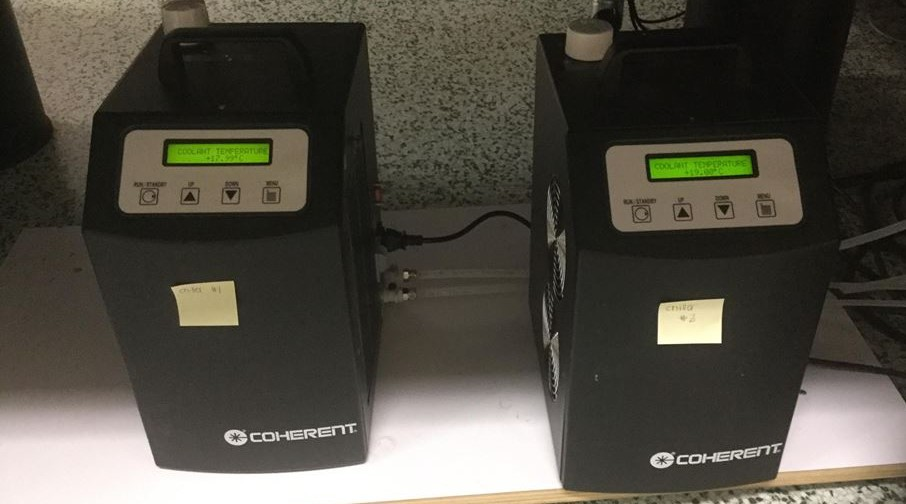
\includegraphics[width=10cm]{cooler.jpg}
        \caption{Refroidisseurs: l'un contrôle le \textit{Verdi}, l'autre le \textit{Mira} et le \textit{RegA}}
        \label{fig:cooler}
        \end{figure}
    \item Peser sur le bouton \textit{Menu}. Vérifier que \textit{Set Temperature} est à 18-19$^\circ$C.
    \item Repeser sur le bouton \textit{Menu}. Attendre que \textit{Coolant Temperature} soit à 18-19$^\circ$C (4-5 minutes).
    \item À l'arrière du \textit{contrôleur Verdi} (voir figure~\ref{fig:controleur-verdi}, mettre l'interrupteur sur \textit{On}).
        \begin{figure}[H]
        \centering
        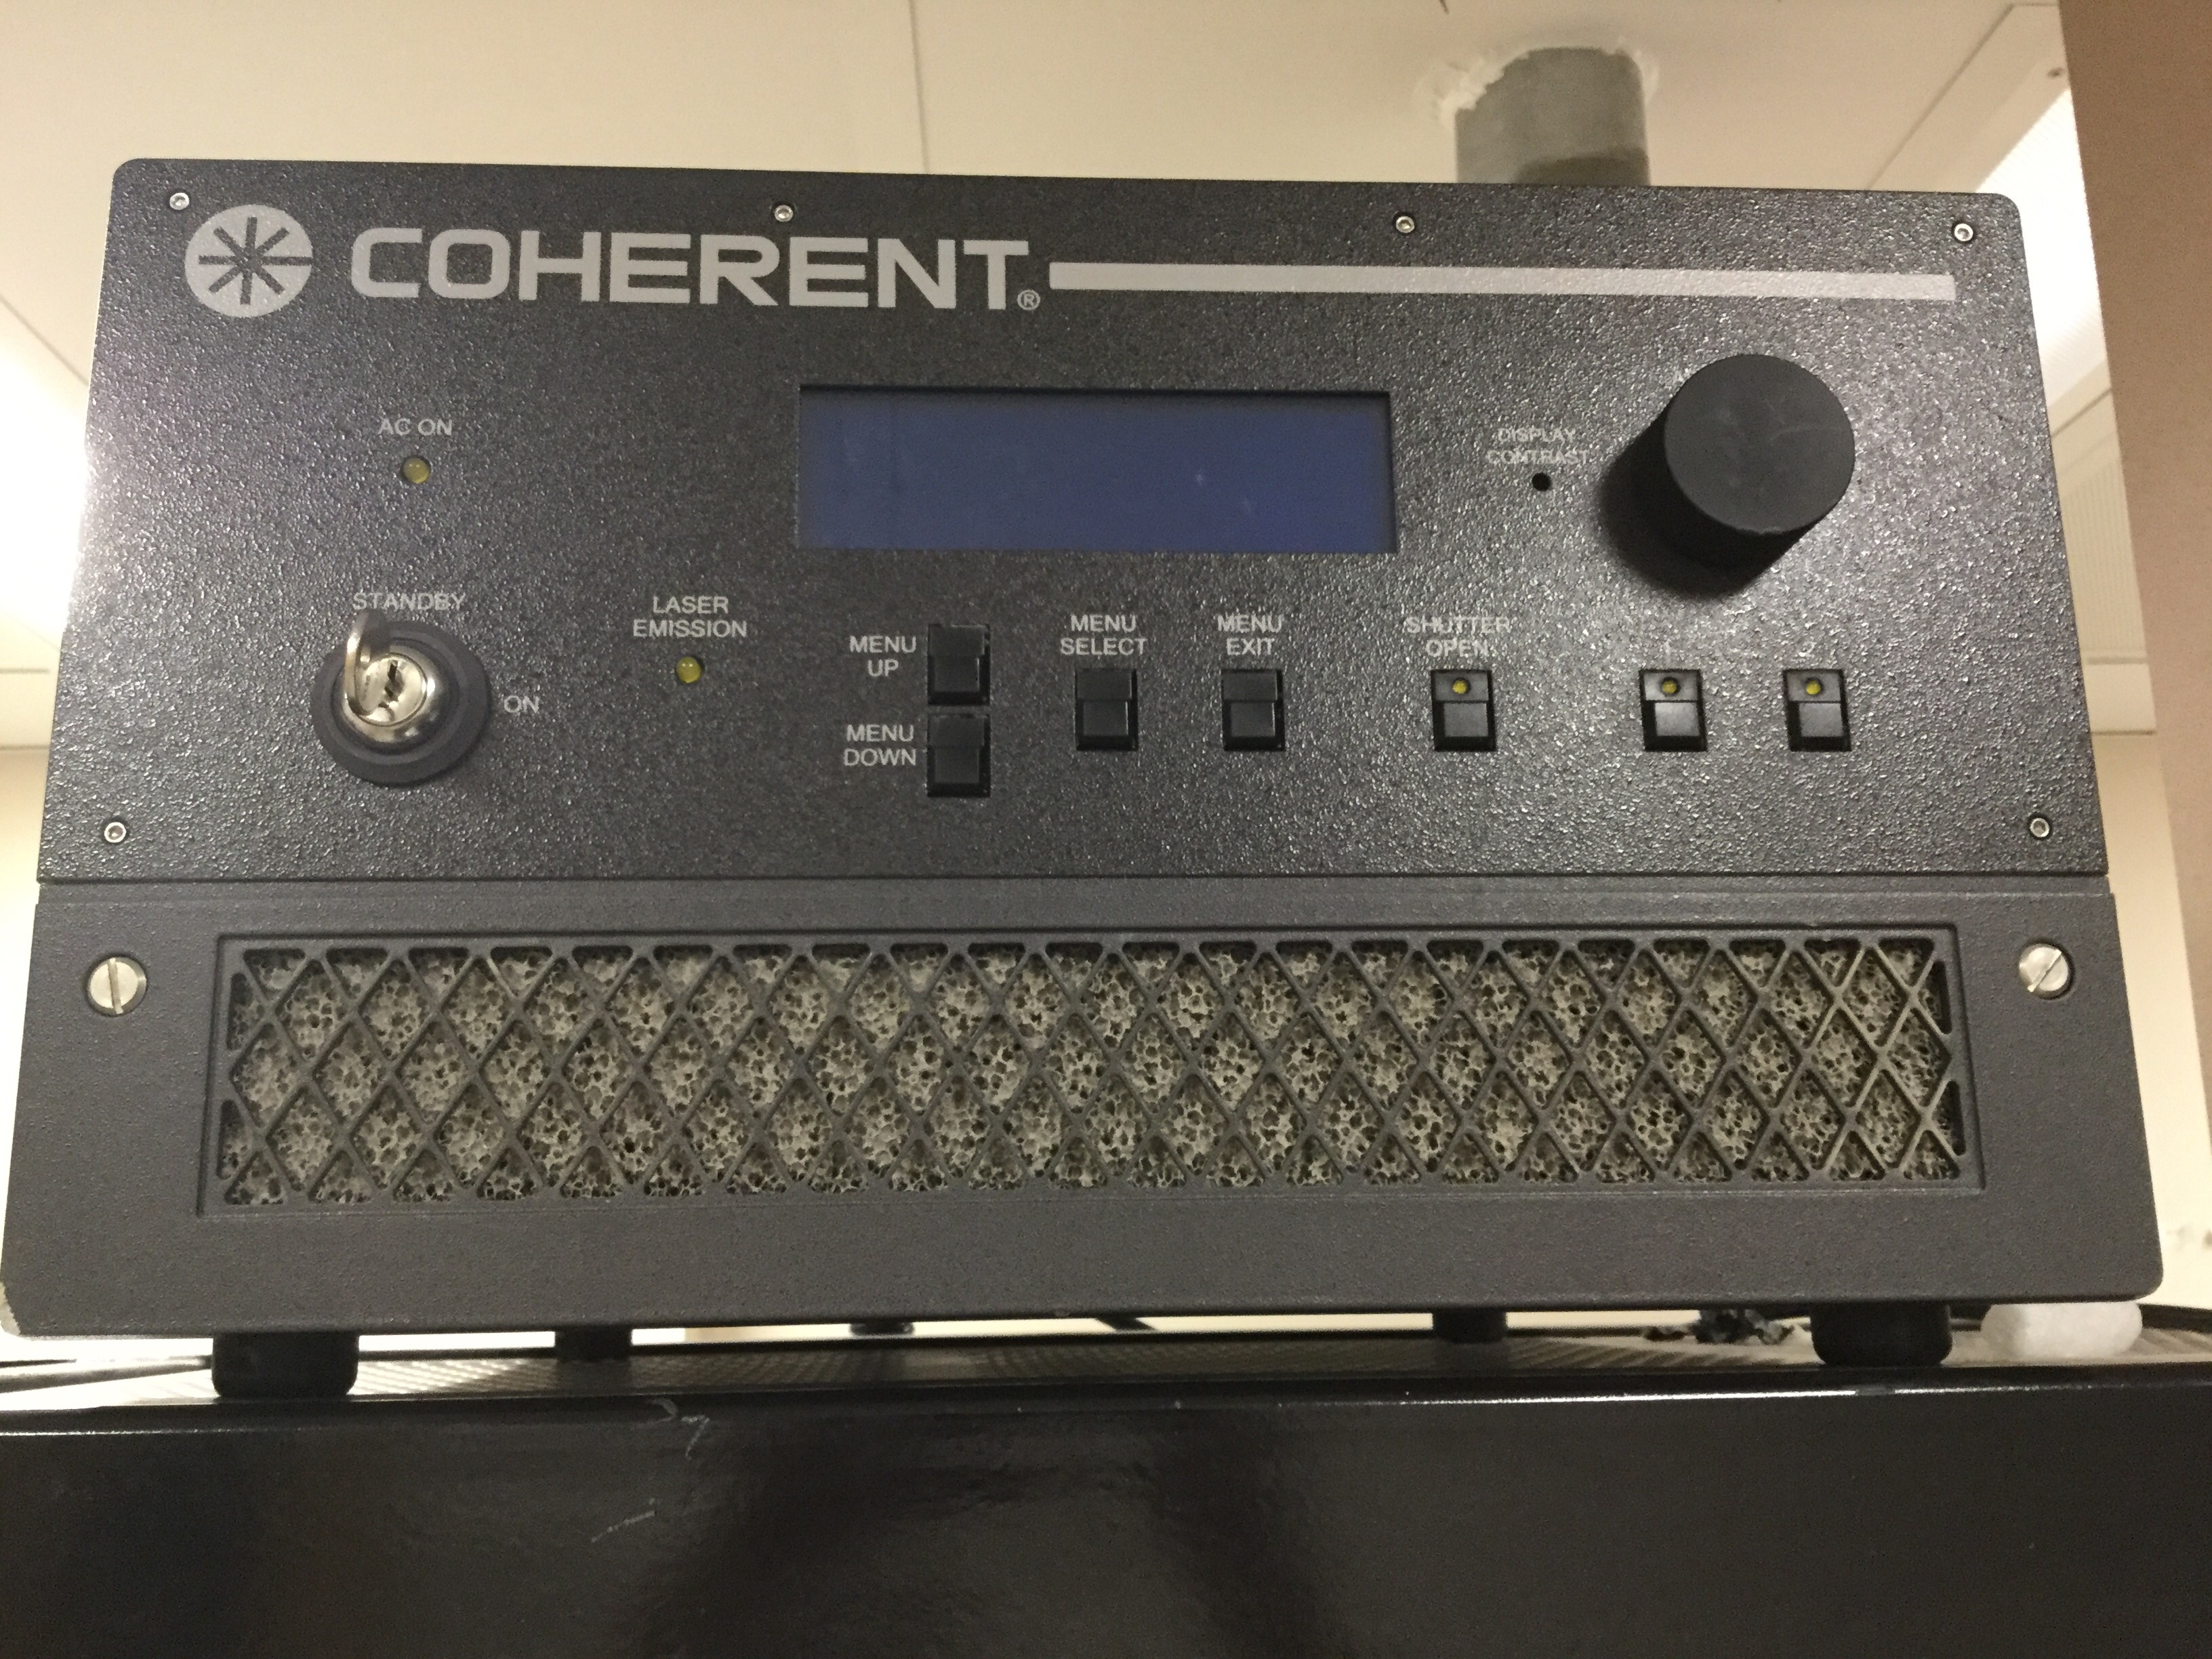
\includegraphics[width=12cm]{controleur-verdi.jpg}
        \caption{Contrôleur du \textit{Verdi}}
        \label{fig:controleur-verdi}
        \end{figure}
    \item Peser sur le bouton \textit{Menu Select}. À l'aide des boutons \textit{Menu Up} et \textit{Menu Down}, aller dans \textit{FAULT Status}. Vérifier que le message affiché est \textit{'SYSTEM OK!'}. Peser sur \textit{Menu Exit}.
    \item Aller dans \textit{LBO Settings}. Vérifier que le message affiché est \textit{'LBO Heating'}. Peser deux fois sur \textit{Menu Exit}.
    \item Vérifier que le message affiché en haut à droite est \textit{'System Warming Up'}.
    \item Tourner la roulette pour ajuster la puissance à 17~W.
    \item Attendre que \textit{'System Warming Up'} soit remplacé par \textit{'Standby'} (environ 10-15 minutes).
\end{enumerate}
\subsection{Allumer le laser}
\label{ssec:allumer_le_laser}
\begin{enumerate}
    \item \label{etape1} Sur le \textit{contrôleur du Verdi} (voir figure~\ref{fig:controleur-verdi}), tourner la clé de \textit{Standby} à \textit{On}.
    \item Allumer la lumière rouge d'avertissement. Il s'agit d'une lumière clignotant à l'extérieur du laboratoire qui avertit avant d'entrer qu'un laser est en marche. Son interrupteur se trouve à côté de la porte d'entrée et est identifié par \textit{'Enseigne lazer en fonction'}.
    \item Attendre que le laser se stabilise (environ 2-3 heures).
    \item Mettre des lunettes de sécurité: OD4 pour une longueur d'onde de 790~nm. 
    \\ Note: Le laser est pulsé et de puissance de plus de 1~W. Il est de classe 4.
    \item Vérifier que les deux refroidisseurs (voir figure~\ref{fig:cooler}) sont environ à 18-19$^\circ$C.
    Si non, remettre à la bonne température à l'aide des boutons \textit{flèches}.
    \item Vérifier s'il y a de l'eau sur la table optique. Si oui, nettoyer le dégât d'eau et remplacer l'eau des refroidisseurs comme expliqué à l'Annexe~\ref{a:chillers}.
    \item Sur le \textit{contrôleur du Verdi} (voir figure~\ref{fig:controleur-verdi}), appuyer sur le bouton \textit{Shutter Open}.
    \item Vérifier que les lumières \textit{AC On}, \textit{Laser Emission} et \textit{Shutter Open} sont allumées.
    \item Vérifier que la \textit{puissance} est d'environ 17~W. Attendre que le \textit{courant} soit d'environ 44~A. Si ces conditions ne sont pas atteintes, remettre la clé sur \textit{Standby}, attendre 1 minute et recommencer à partir de l'étape \ref{etape1}.
\end{enumerate}
\subsection{Ajuster le faisceau laser}
\begin{enumerate}
   \item Si présent, retirer le \textit{beam dump}~(voir figure~\ref{fig:beam-dump}) placé à la sortie du RegA.
        \begin{figure}[H]
        \centering
        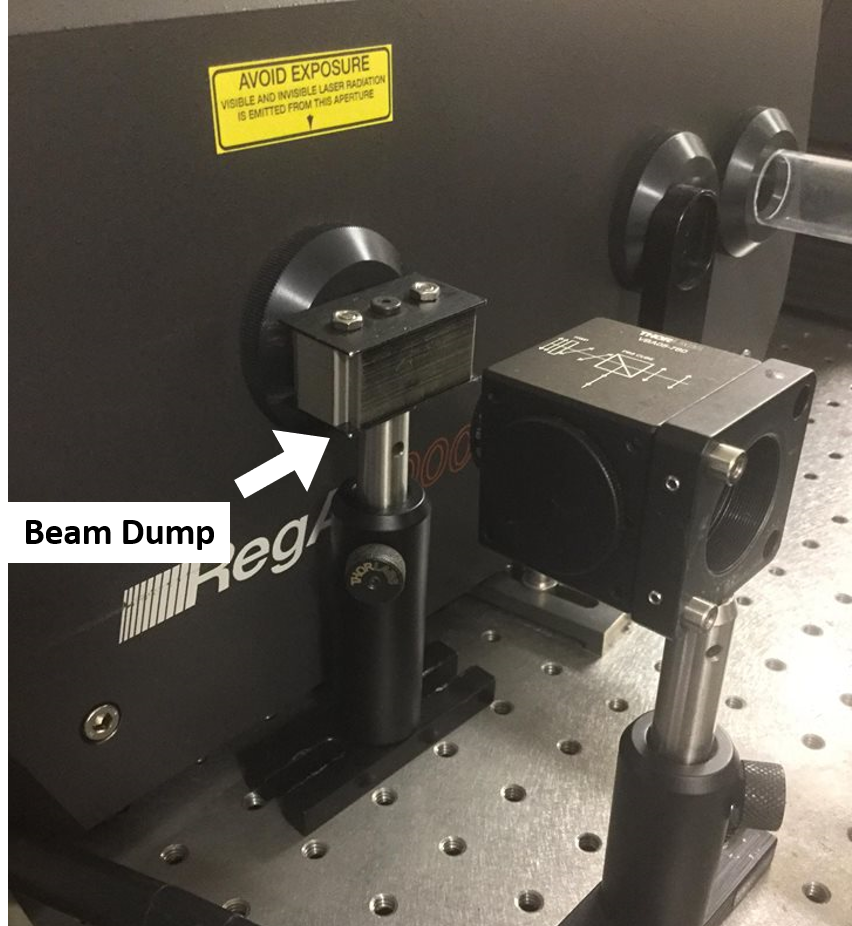
\includegraphics[height=6cm]{beam-dump.png}
        \caption{Beam Dump}
        \label{fig:beam-dump}
        \end{figure}
    \item Tel que montré à la figure~\ref{fig:puissance}, placer le \textit{capteur du puissancemètre} après le \textit{diviseur de puissance}.
        \begin{figure}[H]
        \centering
        \includegraphics[width=15cm]{puissance.png}
        \caption{Mesure de la puissance du laser}
        \label{fig:puissance}
        \end{figure}
    \item Tourner l'\textit{anneau} du \textit{diviseur de puissance} afin d'obtenir une puissance d'environ 750-900~W. Attention:~Le faisceau laser qui sort du RegA ne doit pas revenir sur lui-même. Par conséquent, le \textit{diviseur de puissance} ne doit pas être parfaitement à 90~degrés de la sortie du RegA mais plutôt légèrement tourné (environ 3~degrés) pour que la réflexion soit dirigée ailleurs. On peut le tourner après avoir desserré la vis située sur son pied/base.
    \item Retirer le \textit{capteur} du trajet optique.
        \begin{figure}[H]
        \centering
        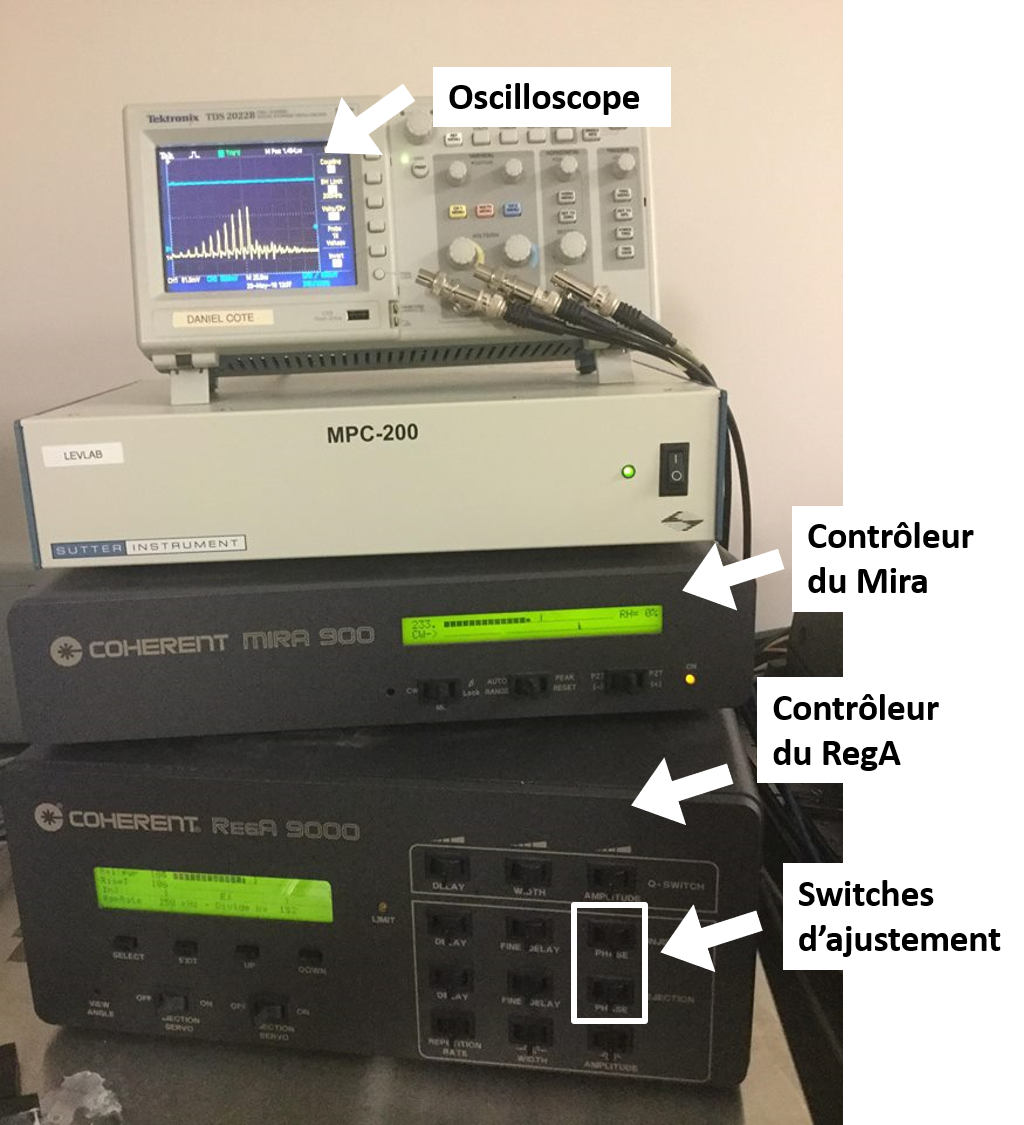
\includegraphics[width=10cm]{controleurs.png}
        \caption{Contrôleurs}
        \label{fig:controleurs}
        \end{figure}
    \item Sur le \textit{contrôleur du Mira} (voir figure~\ref{fig:controleurs}), vérifier que le taux d'humidité (RH) est entre 0\% et 5\%. Si non, augmenter le flux d'azote fourni au système, i.e.:
        \begin{figure}[H]
        \centering
        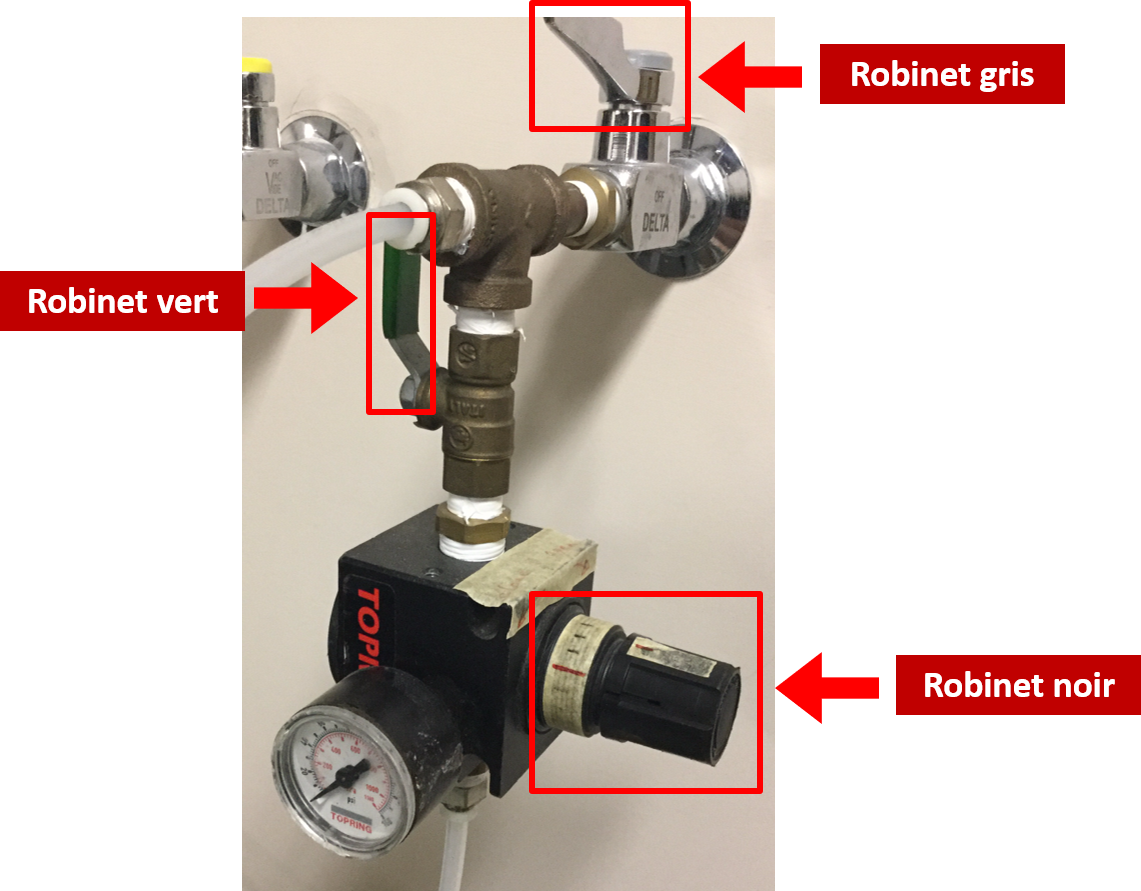
\includegraphics[width=10cm]{azote.png}
        \caption{Alimentation d'azote}
        \label{fig:azote}
        \end{figure}
        \begin{itemize}
        \item[$\bullet$] L'alimentation d'azote se trouve sur le mur juste à côté de la porte d'entrée du laboratoire.
        \item[$\bullet$] Vérifier que le \textit{robinet gris} et le \textit{robinet vert} sont positionnés comme sur la figure~\ref{fig:azote}.
        \item[$\bullet$] Tourner le \textit{robinet noir}, "suffisamment pour entendre le jet quand on approche son oreille et qu'on prête attention, mais le son ne doit pas non plus être trop fort"\footnote{François Côté, 2018}.
        \item[$\bullet$] Une fois le pourcentage d'humidité rétabli, remettre le \textit{robinet noir} à sa position initiale.
        \item[$\bullet$] Si le pourcentage d'humidité demeure élevé, il se peut qu'il y ait une fuite dans le système. Demander l'aide d'un ingénieur/physicien ou d'un superviseur.
        \end{itemize}
    \item Sur le \textit{contrôleur du RegA}, vérifier que la fréquence des impulsions (Rep. Rate) est d'environ 250-260~Hz.
    \item Sur l'\textit{oscilloscope}, vérifier que le signal a une forme semblable à ce qui est montré à la figure~\ref{fig:oscilloscope}. Les chiffres ne sont pas importants.
        \begin{figure}[H]
        \centering
        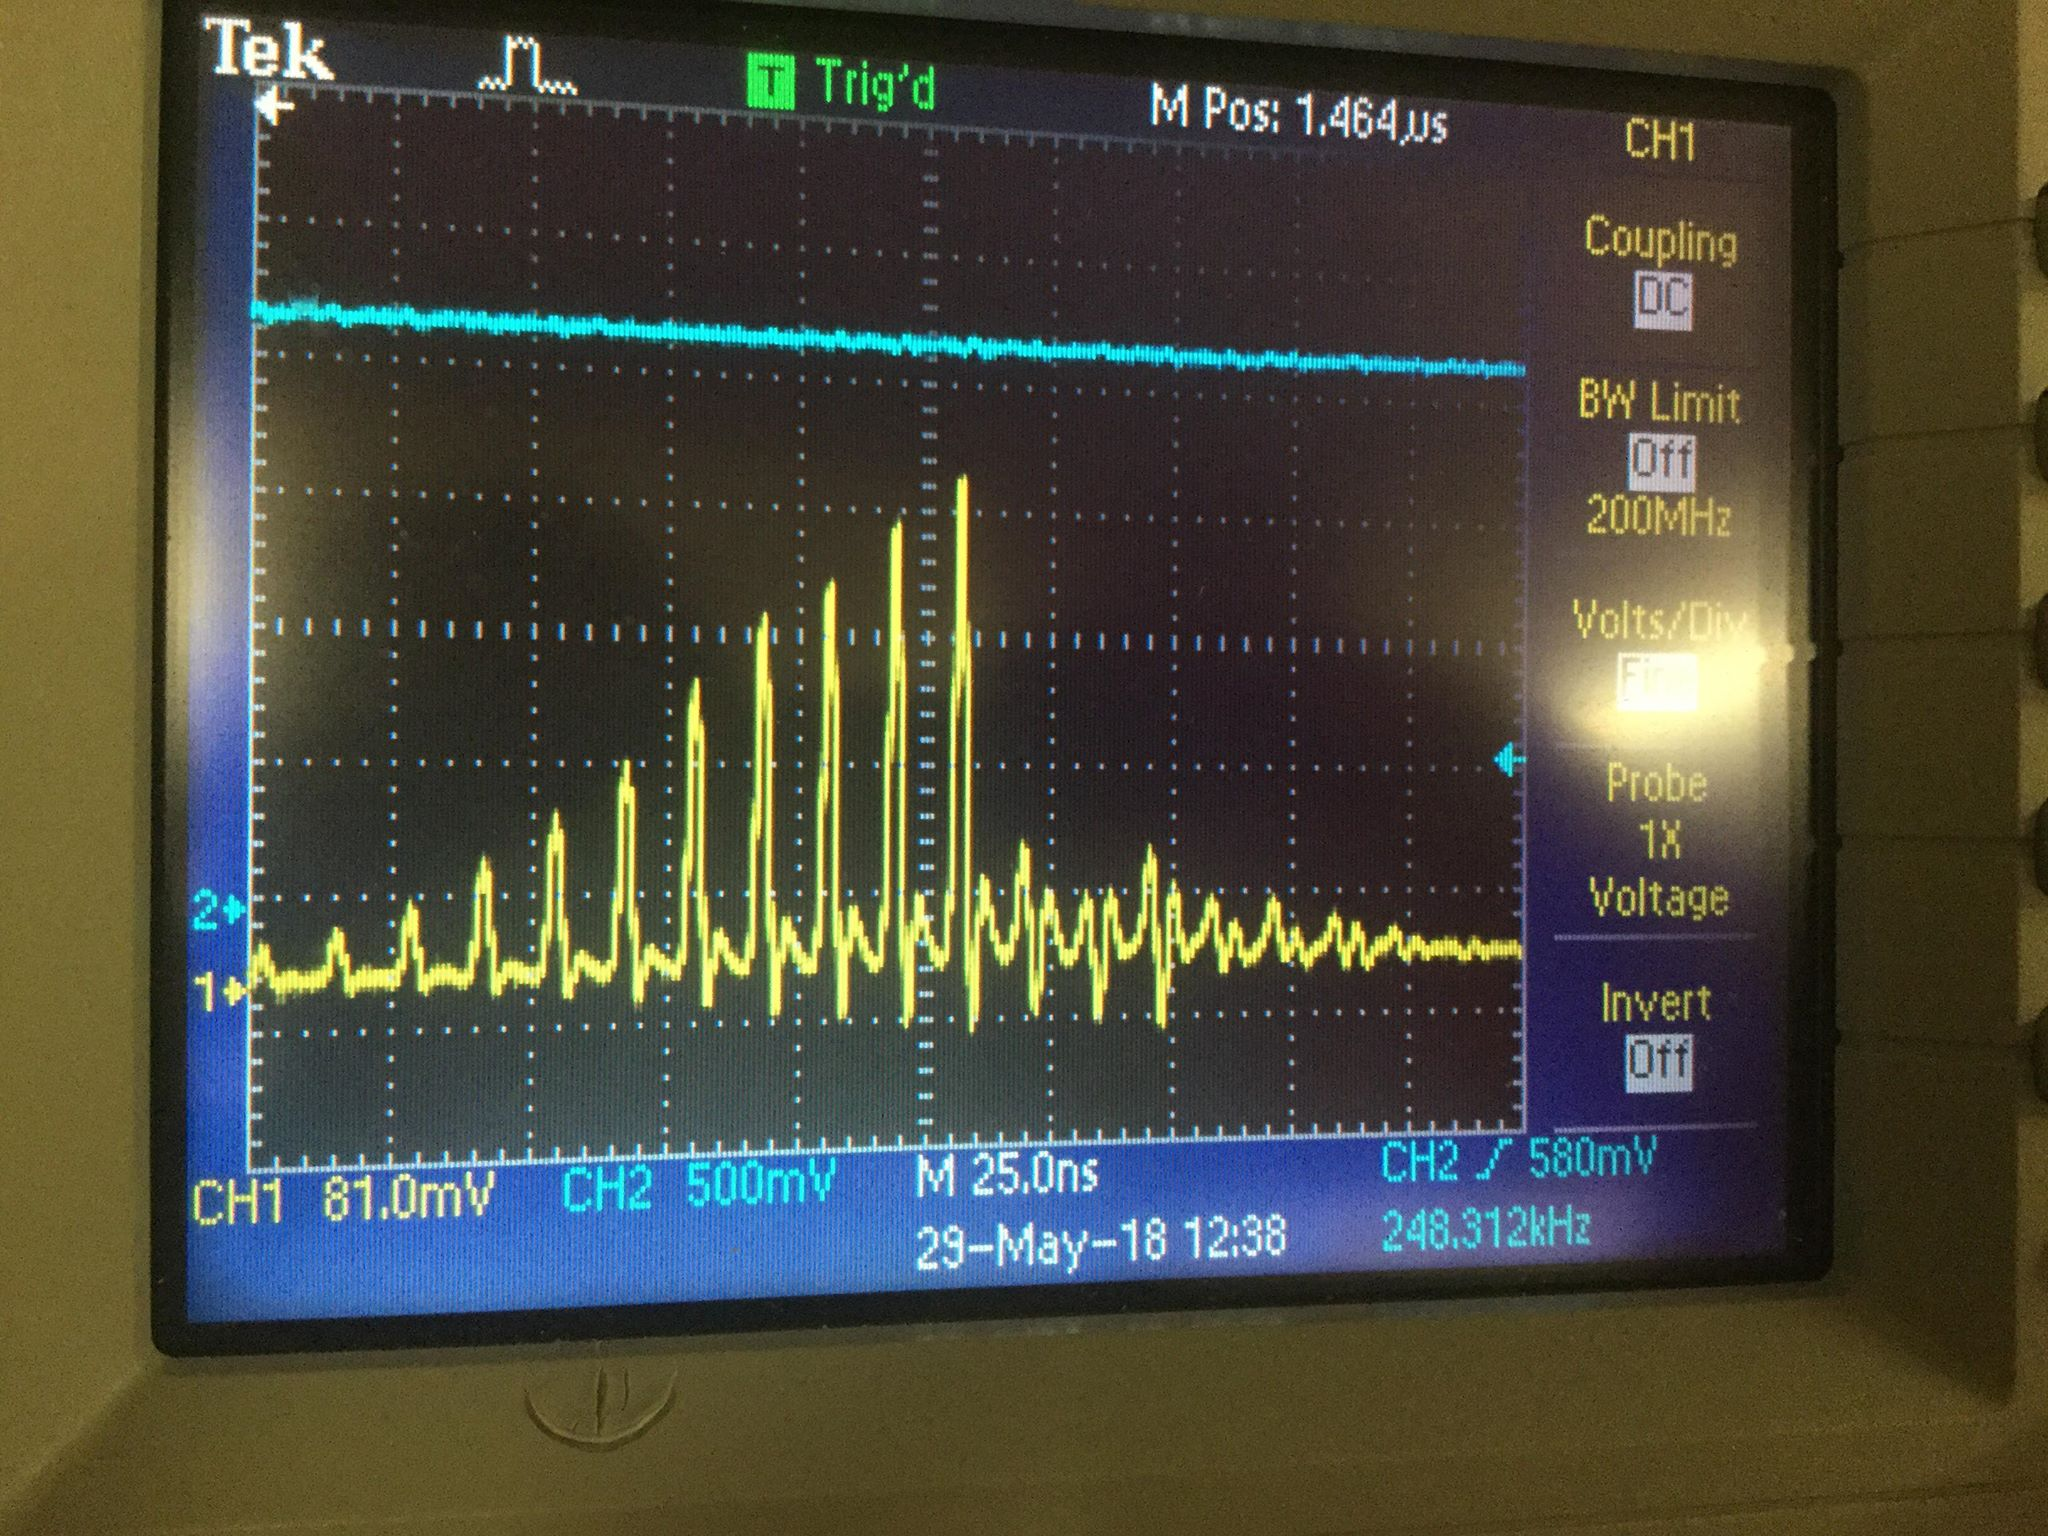
\includegraphics[width=10cm]{oscilloscope.jpg}
        \caption{Signal du laser à l'oscilloscope}
        \label{fig:oscilloscope}
        \end{figure}
    Si non, demander l'aide d'un ingénieur/physicien ou d'un superviseur.
   \item Maximiser la stabilité du signal en ajustant les \textit{switches} (voir figure~\ref{fig:controleurs}). Il ne devrait pas être nécessaire de toucher aux autres boutons des contrôleurs.
   \item A l'aide d'une carte infrarouge, vérifier que le faisceau laser a la forme d'un cercle plein à l'\textit{emplacement A} et d'un anneau à l'\textit{emplacement B} (voir figure~\ref{fig:carte}).
        \begin{figure}[H]
        \centering
        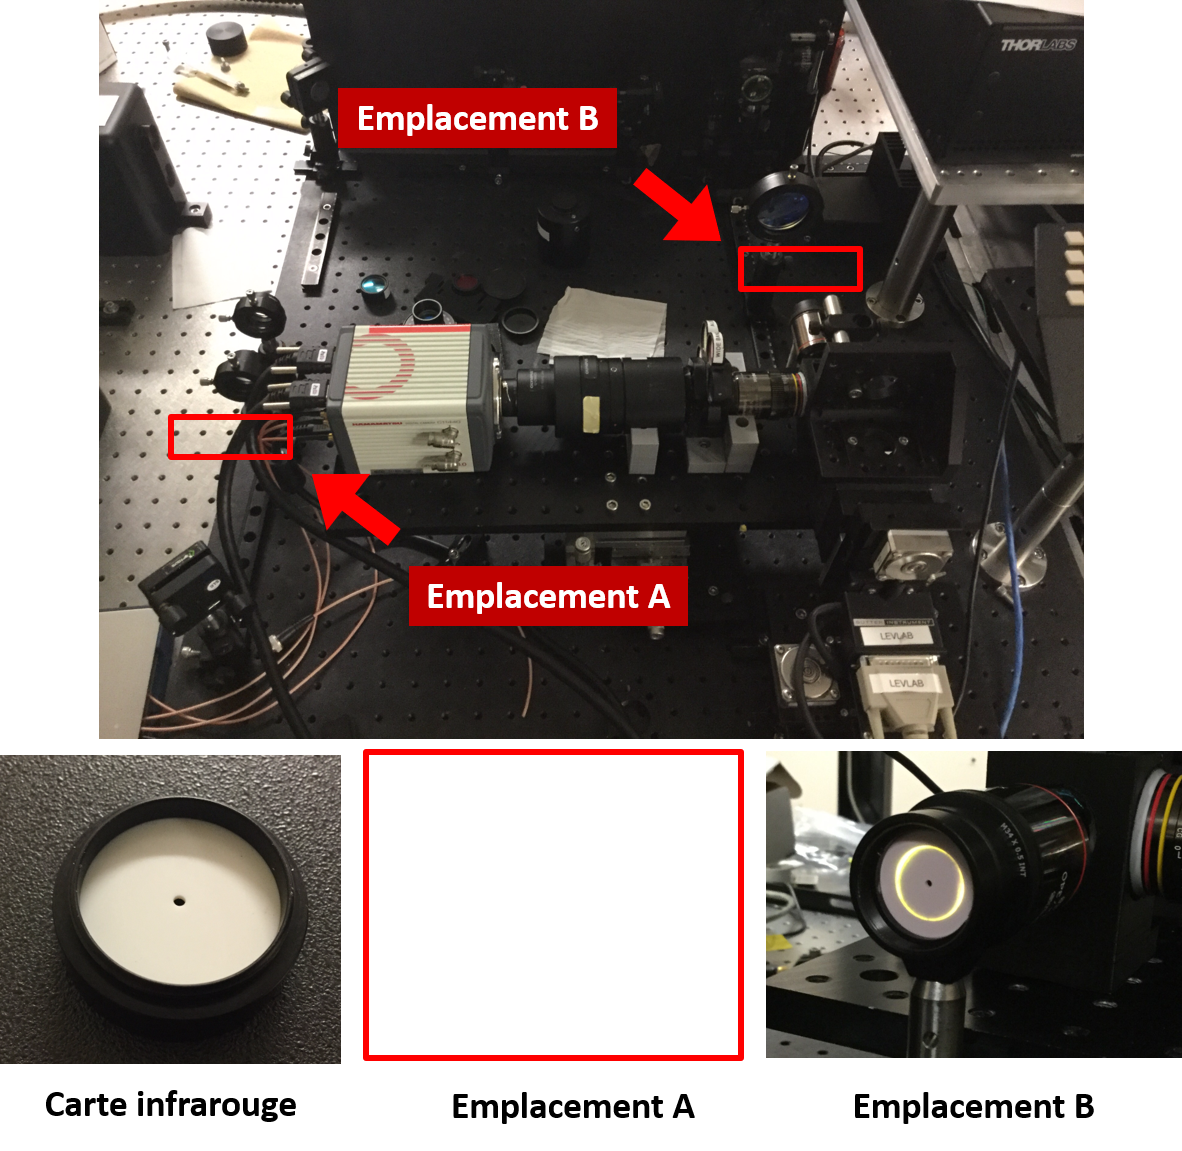
\includegraphics[width=13cm]{carte.png}
        \caption{Carte infrarouge}
        \label{fig:carte}
        \end{figure}
    Si non, il se peut que le trajet optique soit désaligné. Demander l'aide d'un ingénieur/physicien ou d'un superviseur.
   \item Sur le \textit{contrôleur du Mira}, vérifier que le laser n'a pas de composante continue (CW~=~continous wave). Sur la ligne 'Cw->' se trouvent des points '$\ldots$', un ou plusieurs carrés '$\blacksquare$' et une seule barre '|' comme montré à la figure~\ref{fig:cw}.
        \begin{figure}[H]
        \centering
        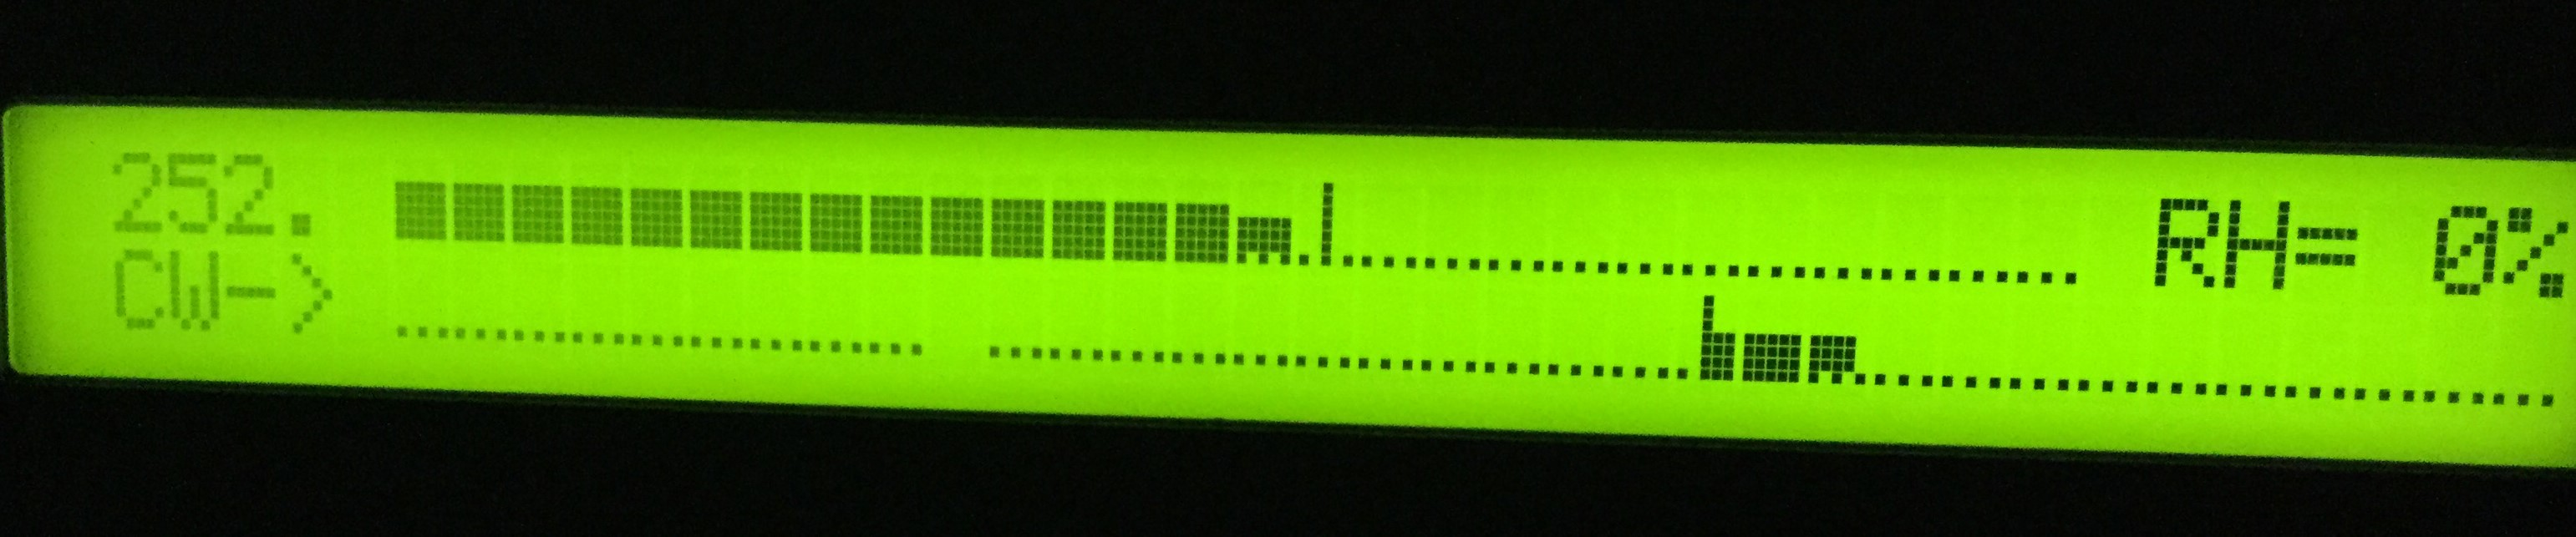
\includegraphics[width=10cm]{cw.jpg}
        \caption{Composante continue du laser}
        \label{fig:cw}
        \end{figure}
   Ajuster l'alignement afin d'avoir un seul \textit{carré} à droite de la \textit{barre}. Pour ce faire, tourner les \textit{vis} identifiées à la figure~\ref{fig:cw_vis}: celles du \textit{RegA} d'abord, puis celles du \textit{Mira} si nécessaire.
        \begin{figure}[H]
        \begin{center} \includegraphics[width=15cm]{cw_vis.png} \end{center}
        \caption{Alignement interne du \textit{RegA} et du \textit{Mira}}
        \begin{footnotesize} Le faisceau laser, pompé par le \textit{Verdi}, passe à travers le \textit{Mira} puis le \textit{RegA}. Les vis sur chacun modifient l'orientation des miroirs à l'intérieur, changeant ainsi l'alignement du laser à la sortie. \end{footnotesize}
        \label{fig:cw_vis}
        \end{figure}
\end{enumerate}
\subsection{Lancer le logiciel d'acquisition}
\begin{enumerate}
    \item Allumer la caméra: mettre l'interrupteur \textit{Power} de \textit{Off} à \textit{On} (voir figure~\ref{fig:cam_power}).
        \begin{figure}[H]
        \centering
        \includegraphics[width=10cm]{cam_power.png}
        \caption{Interrupteur de la caméra}
        \label{fig:cam_power}
        \end{figure}
    \item Ouvrir l'ordinateur Mac.
    \item Entrer dans le compte \textit{dcclab} avec le mot de passe \textit{microscope}.
    \item Ouvrir le logiciel \textit{Umoco} (voir figure~\ref{fig:umoco}). Il y a un raccourci dans la barre de tâches et un autre sur le bureau.
        \begin{figure}[H]
        \centering
        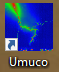
\includegraphics[width=2cm]{umoco.PNG}
        \caption{Raccourci du logiciel \textit{Umoco}}
        \label{fig:umoco}
        \end{figure}
    \item Sur l'interface d'accueil (voir figure~\ref{fig:accueil}), cliquer sur \textit{Camera}. Il est possible que le bouton \textit{Camera} ne soit pas encore disponible: il suffit d'attendre quelques minutes, le temps que le logiciel \textit{Umoco} détecte la caméra.
    \item Mettre \textit{Sensor mode} sur \textit{Area}.
\end{enumerate}
\subsection{Aligner la caméra par rapport au faisceau laser}
\label{ssec:aligner_la_cam}
\begin{enumerate}
    \item Tourner la \textit{roulette de filtres} et sélectionner le \textit{Alexa 594} (voir figure~\ref{fig:filtres}).
        \begin{figure}[H]
        \centering
        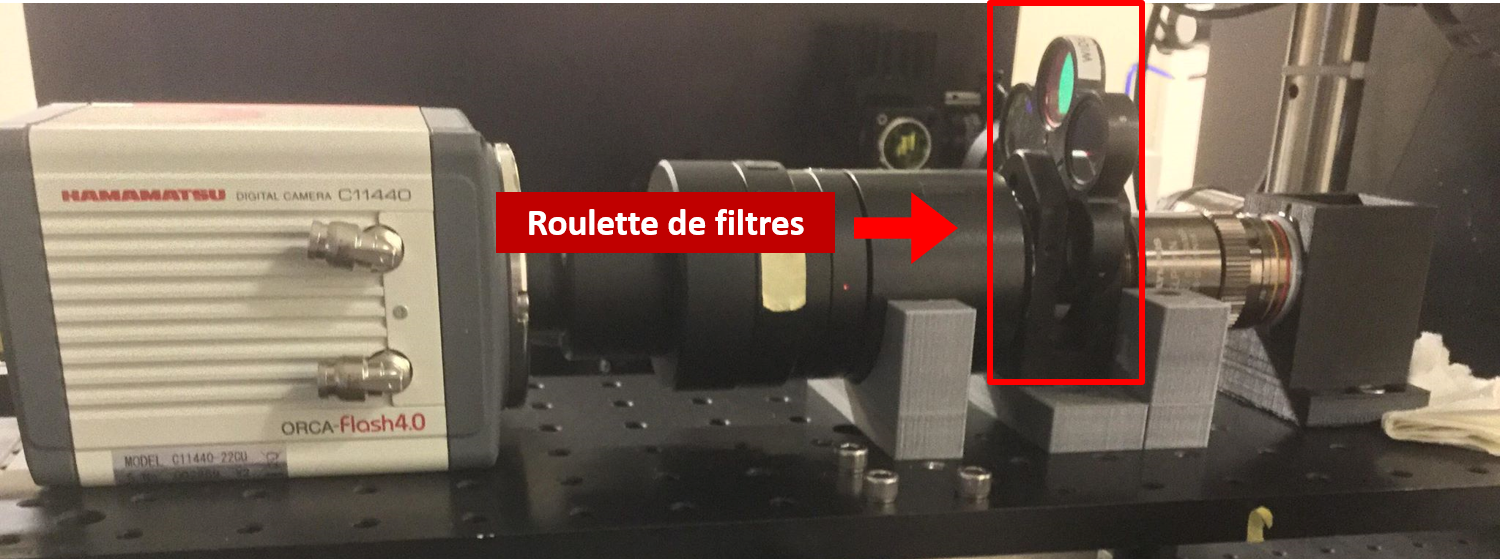
\includegraphics[width=15cm]{filtres.png}
        \caption{Roulette de filtres}
            \begin{footnotesize} \begin{description}[align=right,labelwidth=3cm]
            \item [Wide beam] Pour tout le spectre.
            \item [Alexa 488] Pour le GFP.
            \item [Alexa 568] Pour un fluorophore excité à 568~nm.
            \item [Alexa 594] Pour un fluorophore excité à 594~nm.
            \end{description} \end{footnotesize}
        \label{fig:filtres}
        \end{figure}
    \item Remplir la \textit{chambre} d'eau. En mettre assez pour submerger l'objectif; ne pas trop en mettre au point où la chambre déborderait une fois la cuvette ajoutée (voir figure~\ref{fig:chambre}).
        \begin{figure}[H]
        \centering
        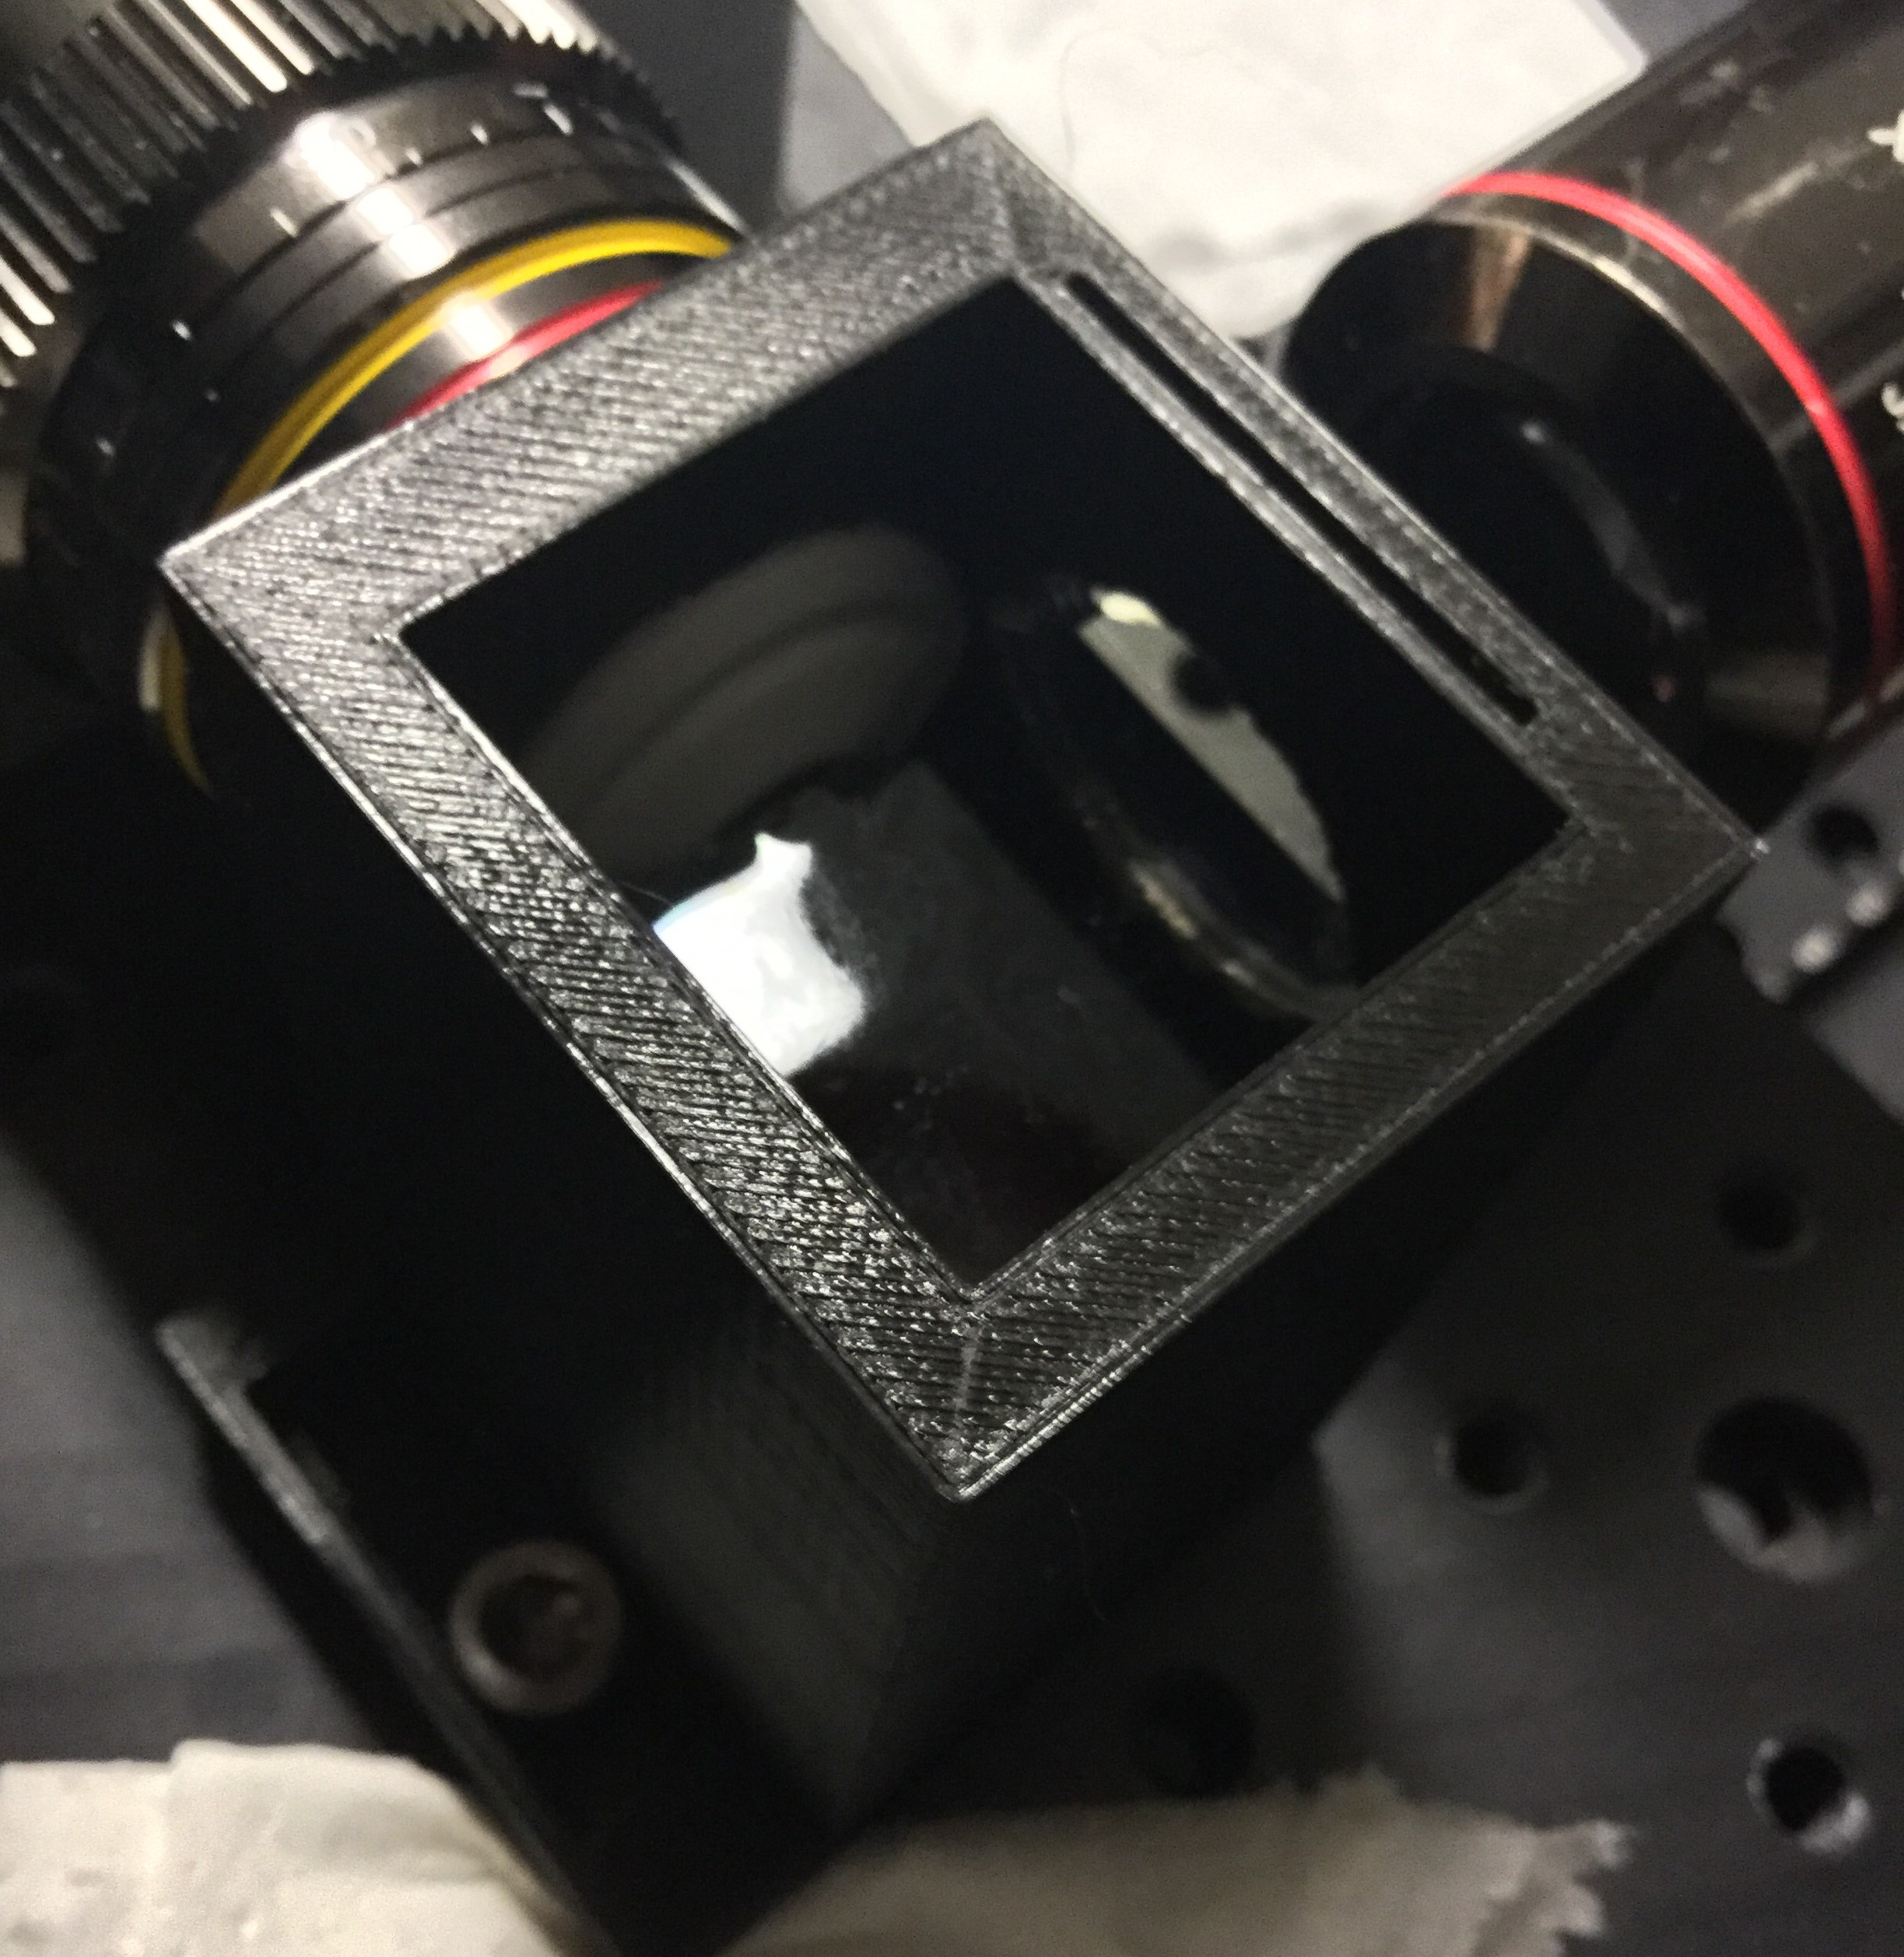
\includegraphics[width=5cm]{chambre.jpg}
        \caption{Chambre: niveau de liquide}
        \label{fig:chambre}
        \end{figure}
    \item Sortir la cuvette de \textit{solution fluorescente} (voir figure~\ref{fig:eau}).
       \begin{figure}[H]
        \centering
        \includegraphics[width=15cm]{eau.png}
        \caption{Substances à utiliser pour l'alignement de la caméra}
        \label{fig:eau}
        \end{figure}
    \item \label{ref1} Insérer cette \textit{cuvette} dans le trou au bout du \textit{support amovible} (voir figure~\ref{fig:suport}). Serrer la \textit{vis noire}.
        \begin{figure}[H]
        \centering
        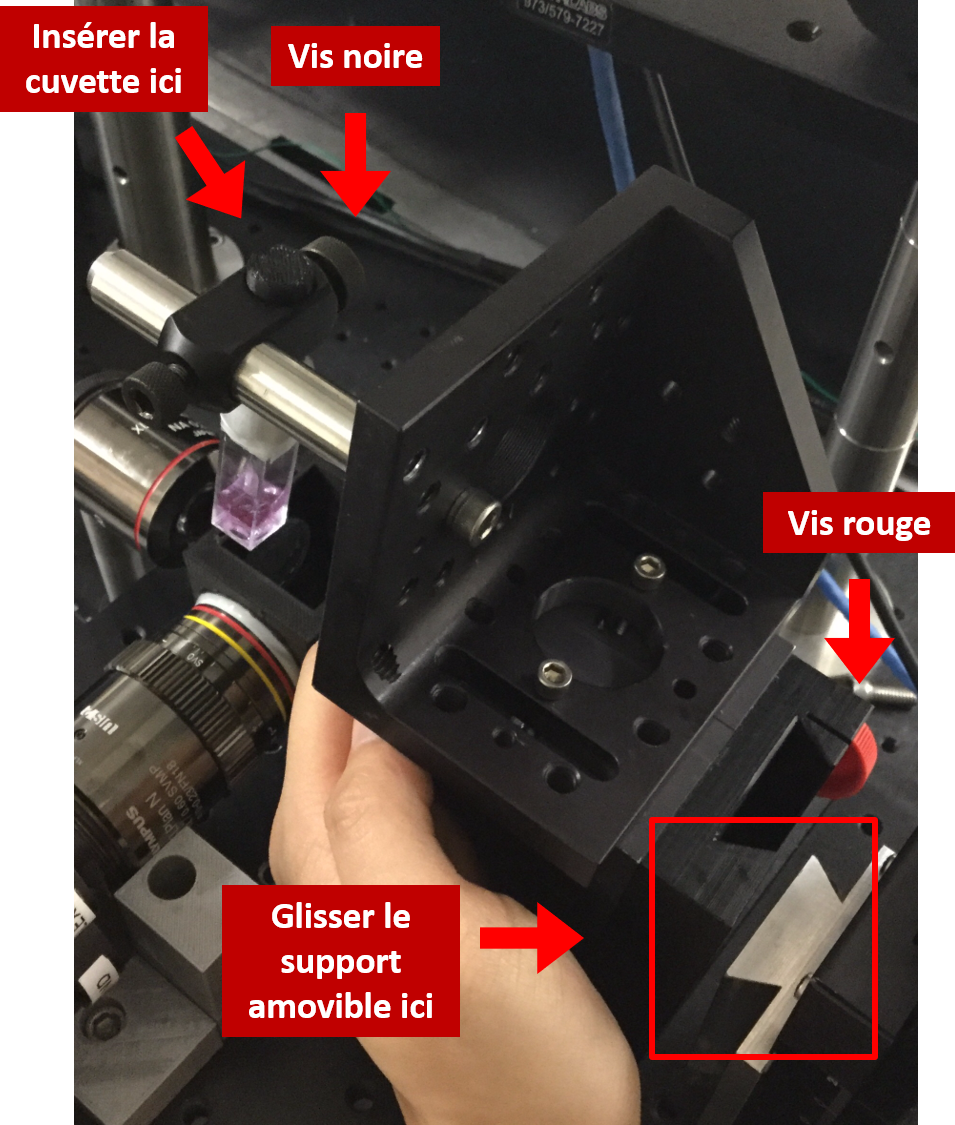
\includegraphics[width=8cm]{support.png}
        \caption{Support amovible}
        \label{fig:suport}
        \end{figure}
    \item Faire glisser le \textit{support amovible} sur la \textit{base motorisée}. Serrer la \textit{vis rouge}.
    \item  \label{ref2} A l'aide des \textit{roulettes} (voir figure~\ref{fig:roulettes}), ajuster la position de l'échantillon.
    \\ But: Voir une ligne fluorescente traverser la cuvette quand on regarde directement à l'oeil.
        \begin{figure}[H]
        \centering
        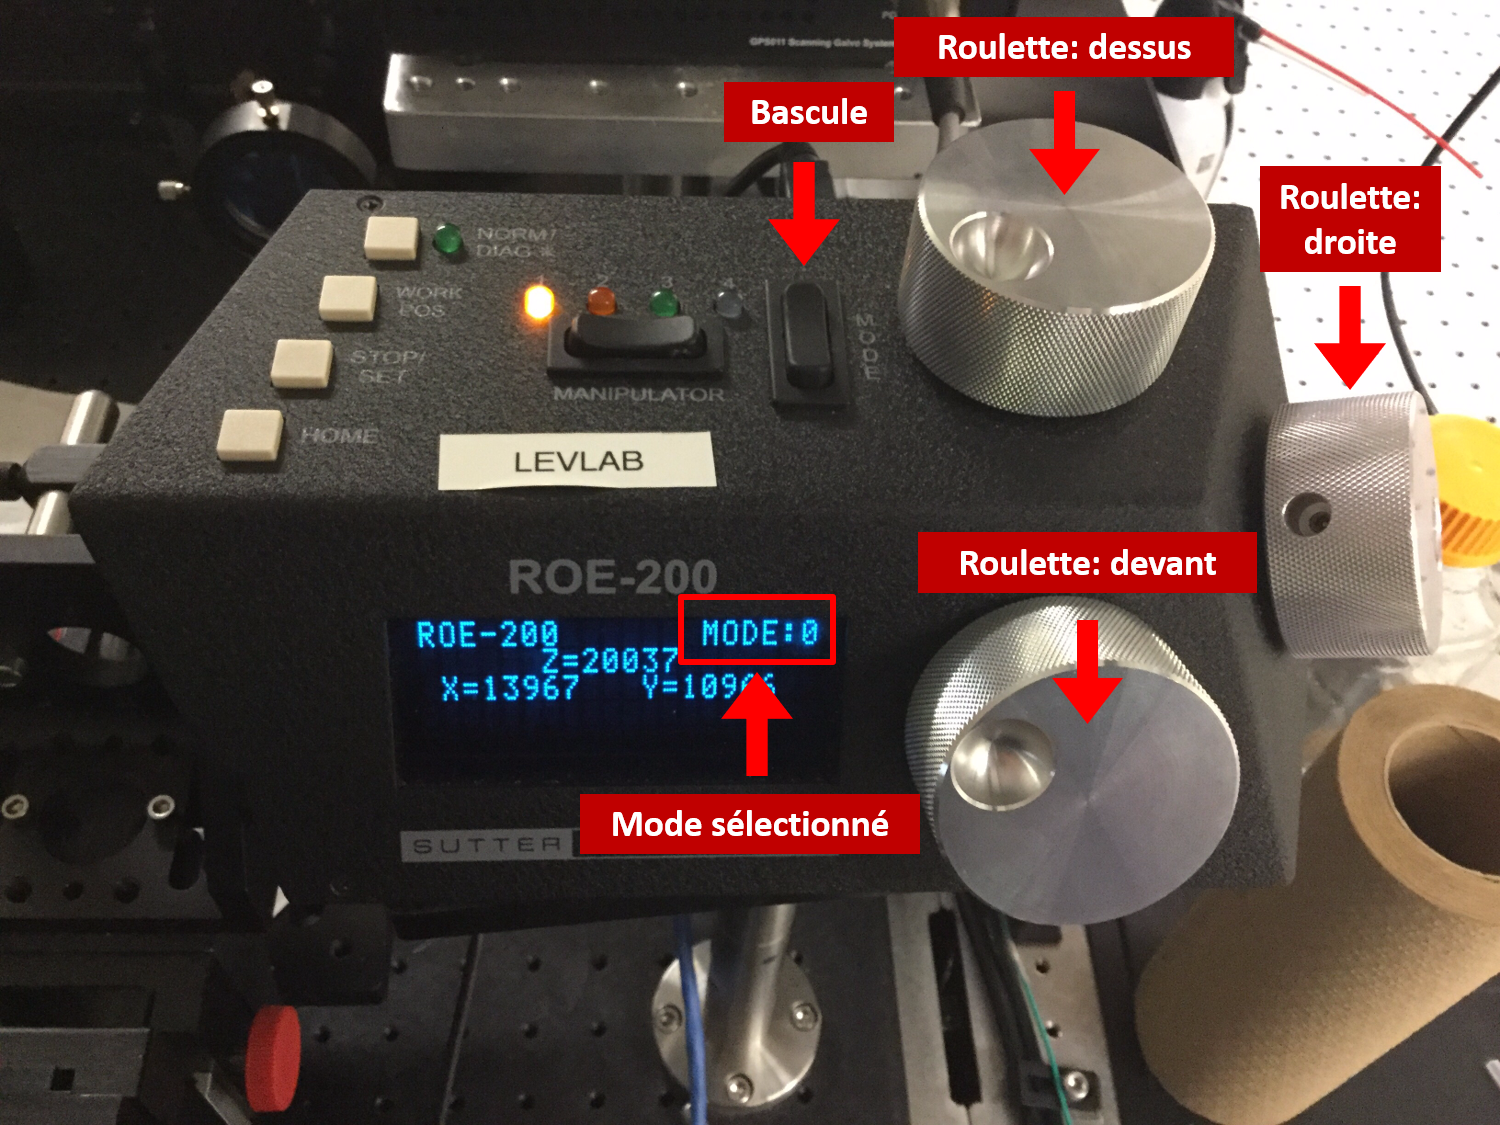
\includegraphics[width=12cm]{roulettes.png}
        \caption{Roulettes de la base motorisée}
            \begin{footnotesize} \begin{description}[align=right,labelwidth=3cm]
            \item [Roulette: dessus] Déplacement vertical. Sens horaire~=~vers le bas.
            \item [Roulette: droite] Déplacement droite-gauche. Sens horaire~=~vers la droite.
            \item [Roulette: devant] Déplacement avant-arrière. Sens horaire~=~vers l'avant.
            \item [***] \textit{Les directions sont données selon le point de vue de la photo.}
            \item [Mode] Le mode va de 0 à 9. 0~=~grands déplacements, 9~=~petits déplacements. \\ \hspace{2.2cm} On peut changer de mode en utilisant la \textit{bascule}.
            \end{description} \end{footnotesize}
        \label{fig:roulettes}
        \end{figure}
    \item Sur l'interface d'accueil (voir figure~\ref{fig:accueil}), cliquer sur \textit{Start Preview} (bouton jaune).
        \begin{figure}[H]
        \centering
        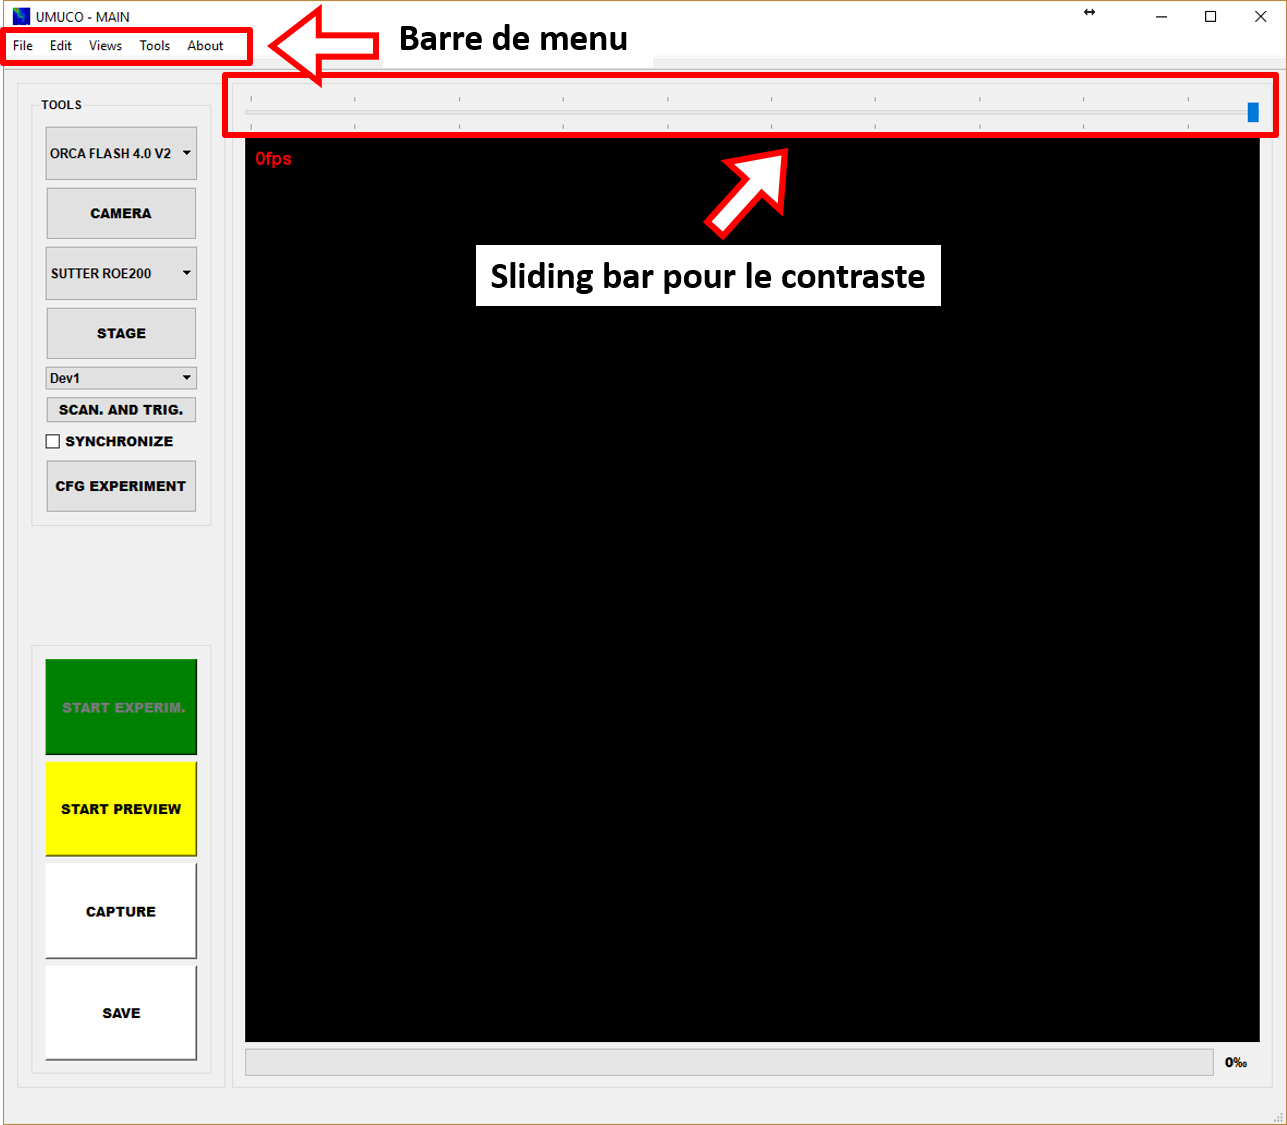
\includegraphics[width=9cm]{accueil.png}
        \caption{Interface du logiciel: accueil}
        \label{fig:accueil}
        \end{figure}
    \item Cliquer sur \textit{Scan. and Trig.} (6e bouton).
    \item Cliquer sur le menu déroulant indiqué à la figure~\ref{fig:tiret}. Sélectionner l'option '-'. Cliquer sur X pour fermer la fenêtre.
        \begin{figure}[H]
        \centering
        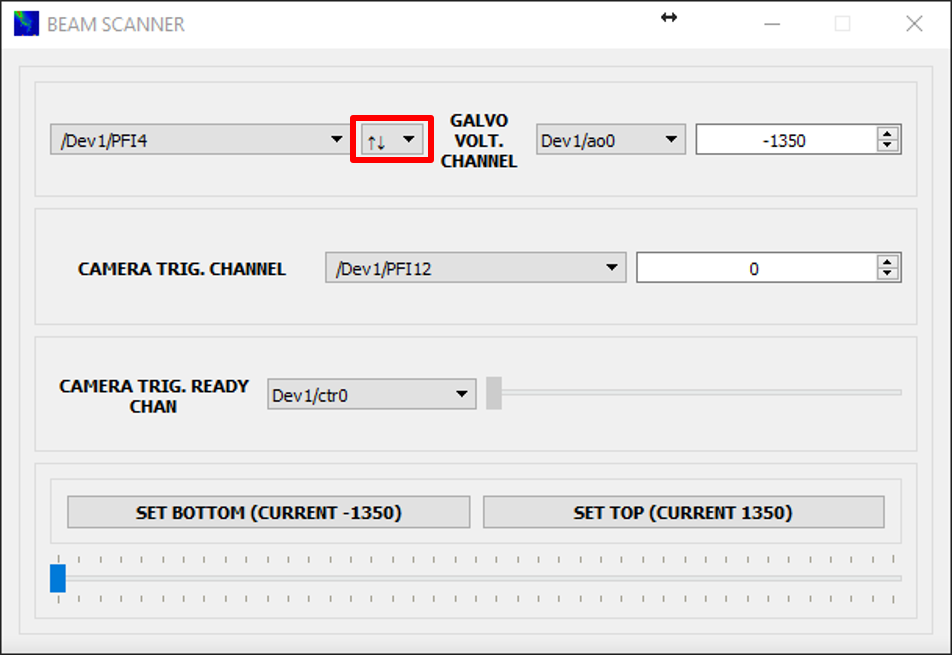
\includegraphics[width=8cm]{tiret.png}
        \caption{Fenêtre pop-up de \textit{Scan. and Trig.}}
        \label{fig:tiret}
        \end{figure}
    \item Sur l'interface d'accueil (voir figure~\ref{fig:accueil}), ajuster le contraste avec la \textit{sliding bar}. Vers la gauche~=~plus de contraste.
    \\ But: Voir du signal à l'écran, i.e. voir des picots de couleur.
        \begin{figure}[H]
        \begin{center}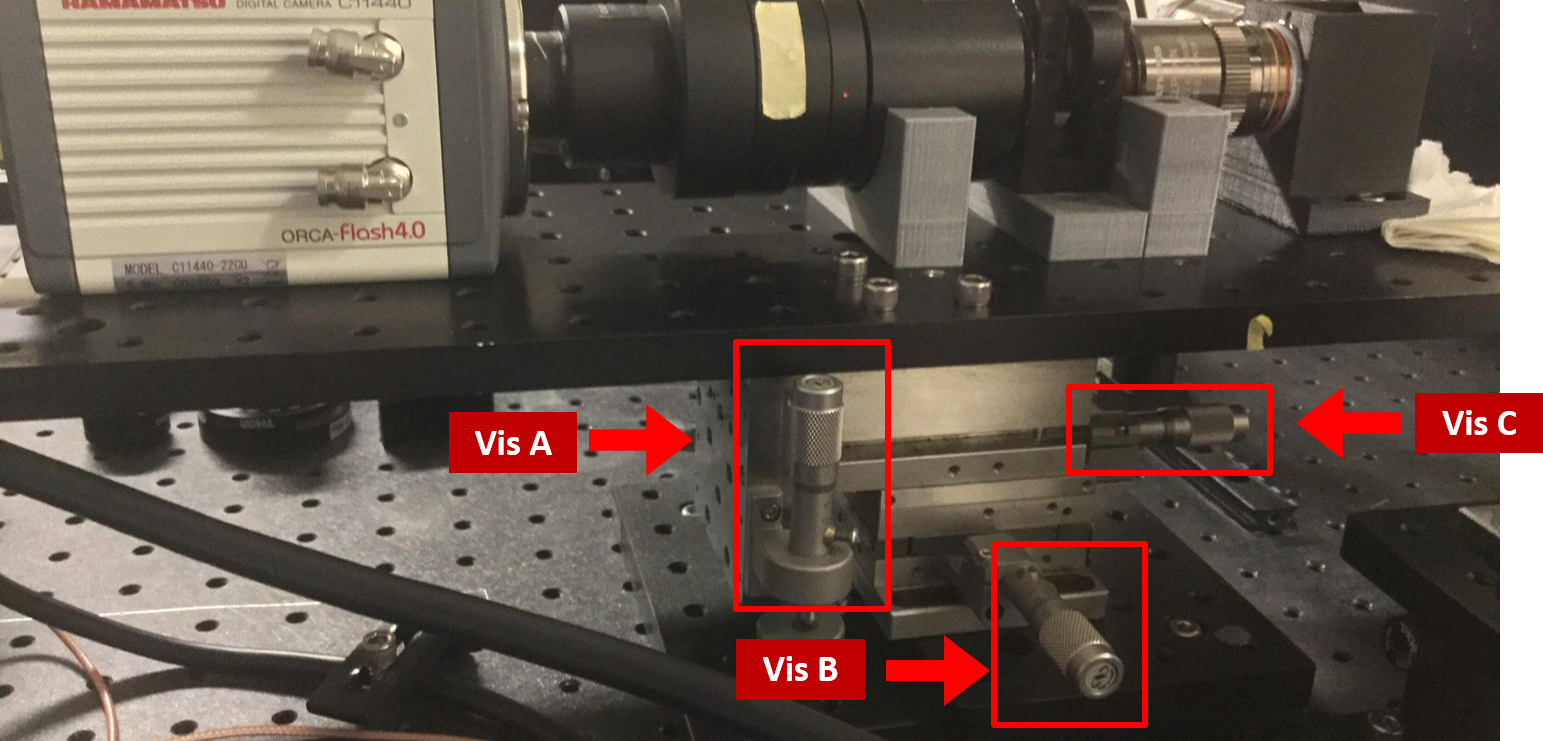
\includegraphics[width=12cm]{vis.png} \end{center}
        \caption{Vis d'ajustement du plateau de la caméra}
            \begin{footnotesize} \begin{description}[align=right,labelwidth=3cm]
            \item [Vis A] Déplacement vertical. Sens horaire~=~monter.
            \item [Vis B] Déplacement horizontal. Sens horaire~=~bouger vers la gauche.
            \item [Vis C] Déplacement en profondeur. Sens horaire~=~reculer.
            \item [***] \textit{Les directions sont données selon le point de vue de la caméra (et non de la photo).}
            \end{description} \end{footnotesize}
        \label{fig:vis}
        \end{figure}
    \item Ajuster la position verticale de la caméra à l'aide de la \textit{vis A} (voir figure~\ref{fig:vis}).
    \\ But: Voir la ligne de fluorescence. La centrer verticalement à l'écran.
    \item Ajuster la position horizontale de la caméra à l'aide de la \textit{vis B}.
    \\ But: Obtenir l'intensité la plus uniforme possible le long de la position horizontale.
    \item Ajuster la position en profondeur de la caméra à l'aide la \textit{vis C}.
    \\ But: Avoir la ligne de fluorescence au focus, i.e. avoir la ligne la plus nette/fine possible.
    \item S'aider des outils d'alignement: Dans la \textit{barre de menu} de l'interface logiciel (voir figure~\ref{fig:accueil}), cliquer sur \textit{Tools} et sur \textit{Alignment tools}.
        \begin{figure}[H]
        \centering
        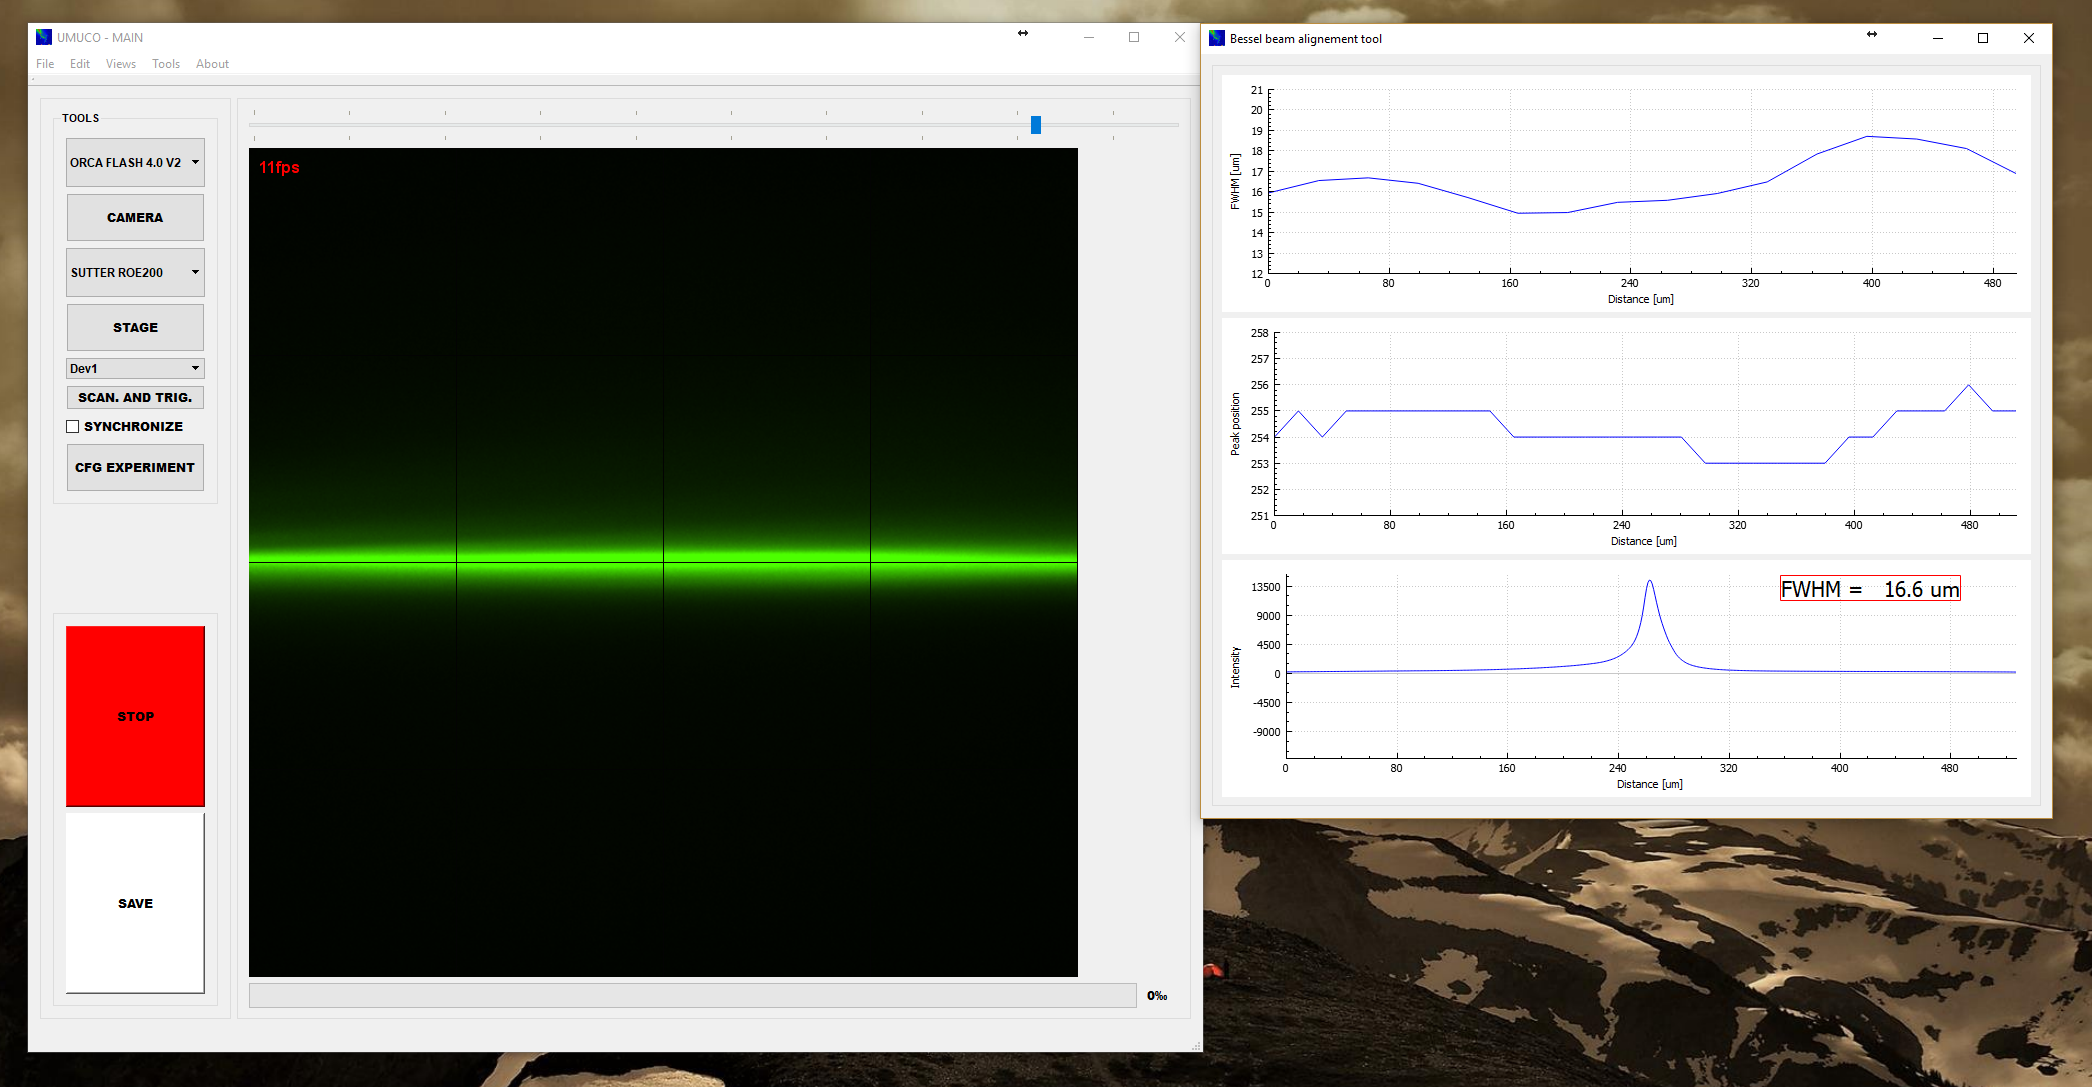
\includegraphics[width=\linewidth]{alignement.PNG}
        \caption{Outils d'alignement}
        \label{fig:alignement}
        \end{figure}
        \begin{description}[align=left,labelwidth=3cm]
        \item [FWHM against Distance] montre la largeur à mi-hauteur du profil d'intensité selon la position axiale (i.e. le long du faisceau). But: avoir une fonction constante. On peut ajuster en tournant la \textit{vis B}.
        \item [Peak Position against Distance] montre la position verticale du pic d'intensité selon la position axiale (i.e. le long du faisceau). Autrement dit, on voit si le faisceau est droit/parallèle horizontalement par rapport à la caméra. But: avoir une fonction constante. On peut ajuster en tournant la vis du bas du miroir présenté à la figure~\ref{fig:miroir}.
            \begin{figure}[H]
            \centering
            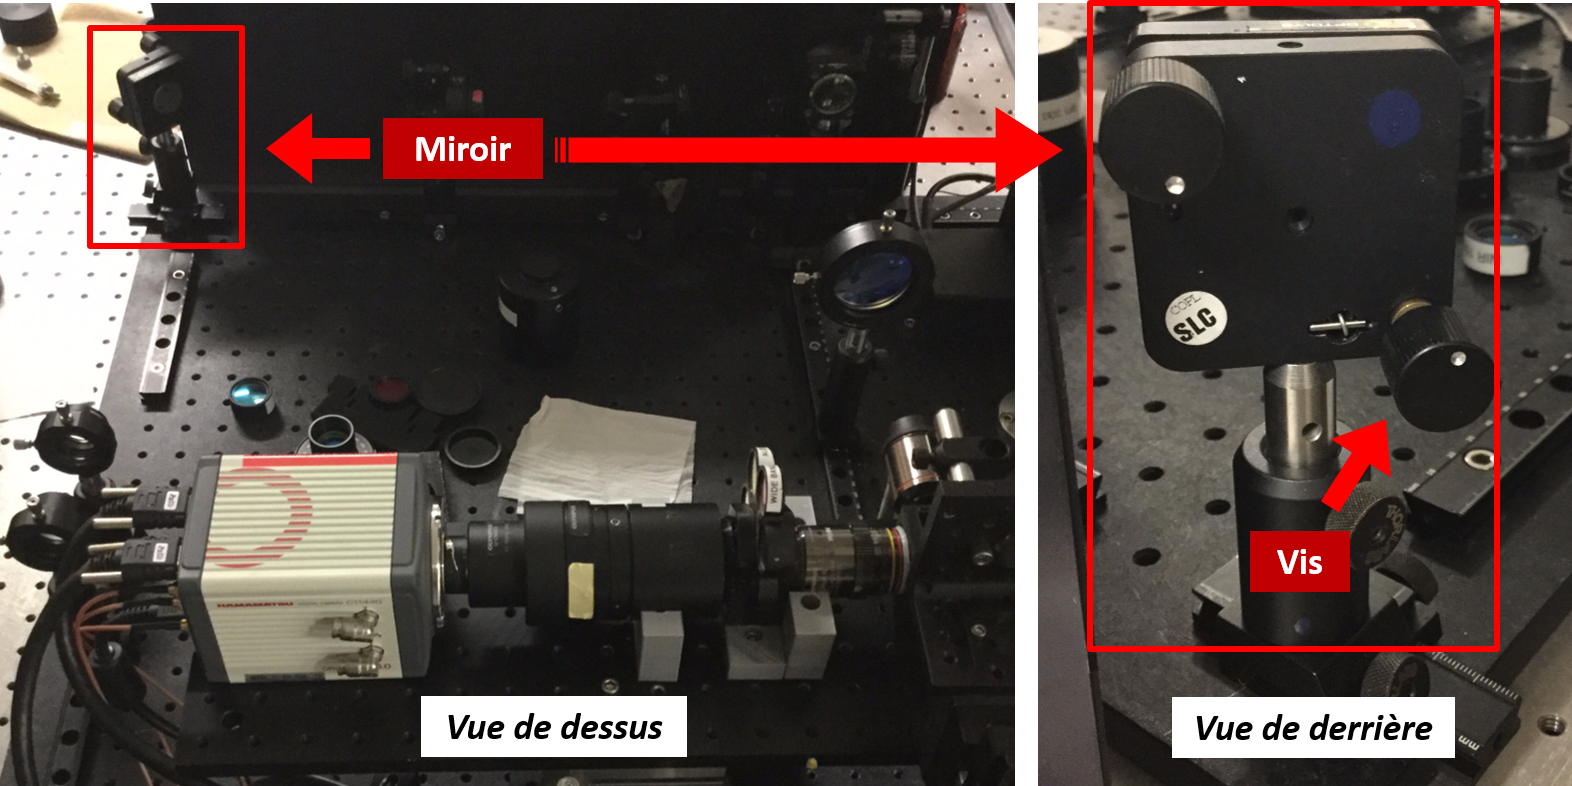
\includegraphics[width=15cm]{miroir.png}
            \caption{Miroir à ajuster}
            \label{fig:miroir}
            \end{figure}
        \item [Intensity against Distance] montre l'intensité selon la position verticale. Autrement dit, on voit le profil d'intensité du faisceau. But: avoir le pic le plus symétrique et étroit possible. La valeur du FWHM (largeur à mi-hauteur) de la courbe sur le graphique est également affichée; on veut le chiffre le plus petit. On peut ajuster en utilisant les \textit{vis B} et \textit{C}.
        \end{description}
    \item Cliquer sur X pour fermer la fenêtre d'outils d'alignement.
\end{enumerate}
\subsection{Saisir les paramètres de scan du faisceau}
\begin{enumerate}
    \item Cliquer sur \textit{Scan. and Trig.} (6e bouton).
    \item Cliquer sur le menu déroulant indiqué à la figure~\ref{fig:tiret}. Sélectionner l'option '$\uparrow\downarrow$'.
    \item Au besoin, ajuster le contraste.
    \item Taper '1000' à l'endroit indiqué à la figure~\ref{fig:courant}. Cette valeur correspond au courant envoyé au galvanomètre. Cliquer sur \textit{Set Top (current \#\#\#\#)}. Il devrait y avoir un bande noire en haut de l'écran.
        \begin{figure}[H]
        \centering
        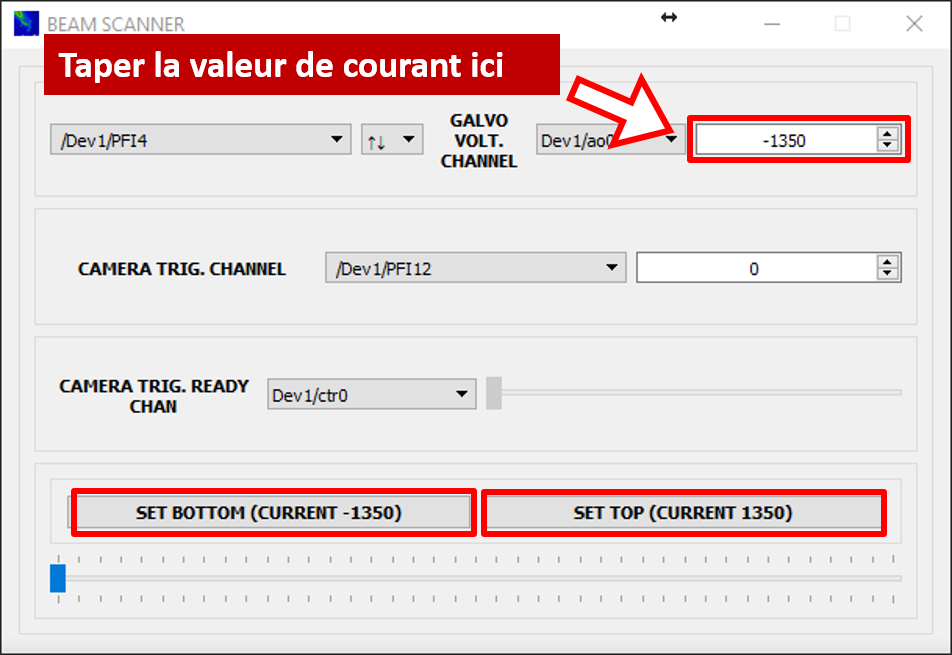
\includegraphics[width=10cm]{current.png}
        \caption{Fenêtre pop-up \textit{Scan. and. Trig.}}
        \label{fig:courant}
        \end{figure}
    \item Taper '1100' et cliquer sur \textit{Set Top (current 1000)}. Noter que la bande noire est plus étroite.
    \item Répéter l'étape précédente jusqu'à ce que la bande noire disparaisse. On veut que la bande lumineuse se rende jusqu'au rebord de l'écran sans toutefois trop dépasser. Trop dépasser entraîne une perte de puissance (i.e. fluorescence non captée par la caméra) et une acquisition de données plus longue. La valeur du courant est normalement entre 1200 et 1400.
    \item Sélectionner la limite inférieure de courant de la même façon que la limite supérieure vient d'être sélectionnée. Taper la valeur dans la même boîte. Attention: la valeur est négative; elle est normalement entre -1400 et -1200. Utiliser le bouton \textit{Set Bottom (current \#\#\#\#)}.
    \item Cliquer sur X pour fermer la fenêtre.
\end{enumerate}
\subsection{Préparer l'échantillon}
\begin{center} $\ast\ast\ast$ Local F-6451 $\ast\ast\ast$ \end{center}
\begin{enumerate}
    \item Tiroir du haut: sortir le contenant en plastique identifié \textit{Stock imagerie Lightsheet}.
    \item Prendre une cuvette propre.
    \item Sortir avec soin l'échantillon de son contenant d'origine et le placer dans le fond de la cuvette.
    \item Si nécessaire, stabiliser l'échantillon (voir figure~\ref{fig:pipette}).
        \begin{figure}[H]
        \begin{center} 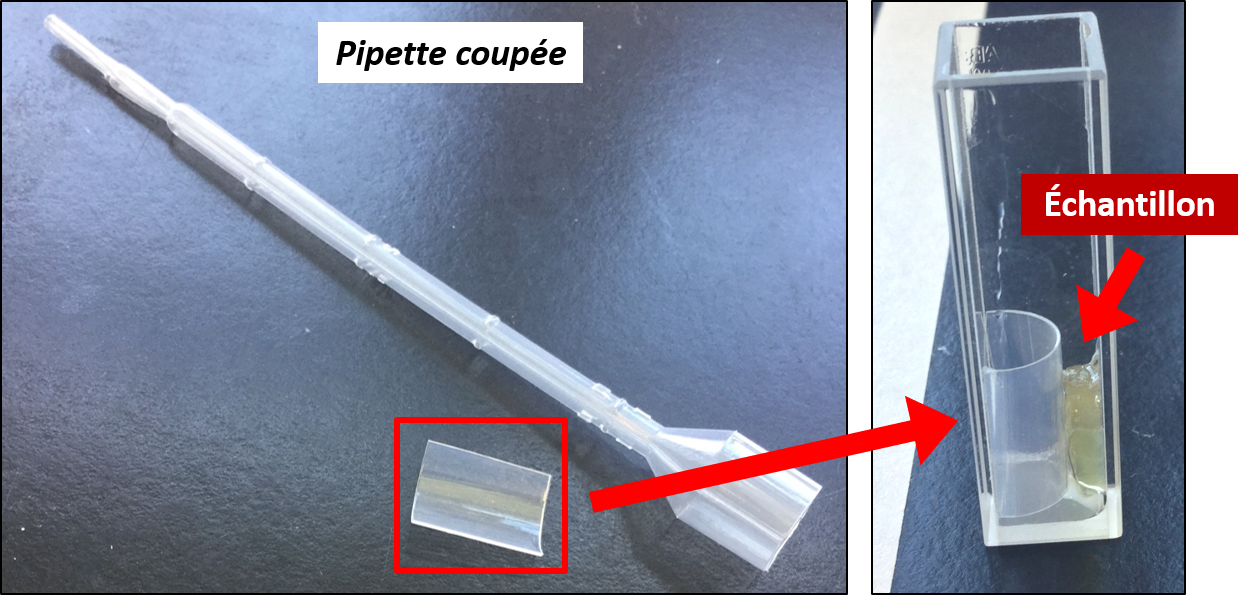
\includegraphics[width=13cm]{pipette.png} \end{center}
        \caption{Exemple de stabilisation de l'échantillon dans la cuvette}
        \begin{footnotesize} Ici, on a une tranche de mésencéphale. On coupe une pipette et on insère le morceau de plastique courbé dans la cuvette. \end{footnotesize}
        \label{fig:pipette}
        \end{figure}
    \item Verser la solution du contenant d'origine dans la cuvette.
    \item Vérifier si l'échantillon est complètement immergé. Si non, ajouter de la solution (même que celle utilisée pour le dernier traitement de la méthode de clarification).
    \item Vérifier qu'il n'y a pas de bulles, de corps étrangers ou autres dans la cuvette.
    \item Mettre le bouchon et sceller avec de la parafilm (voir figure~\ref{fig:parafilm}).
        \begin{figure}[H]
        \centering
        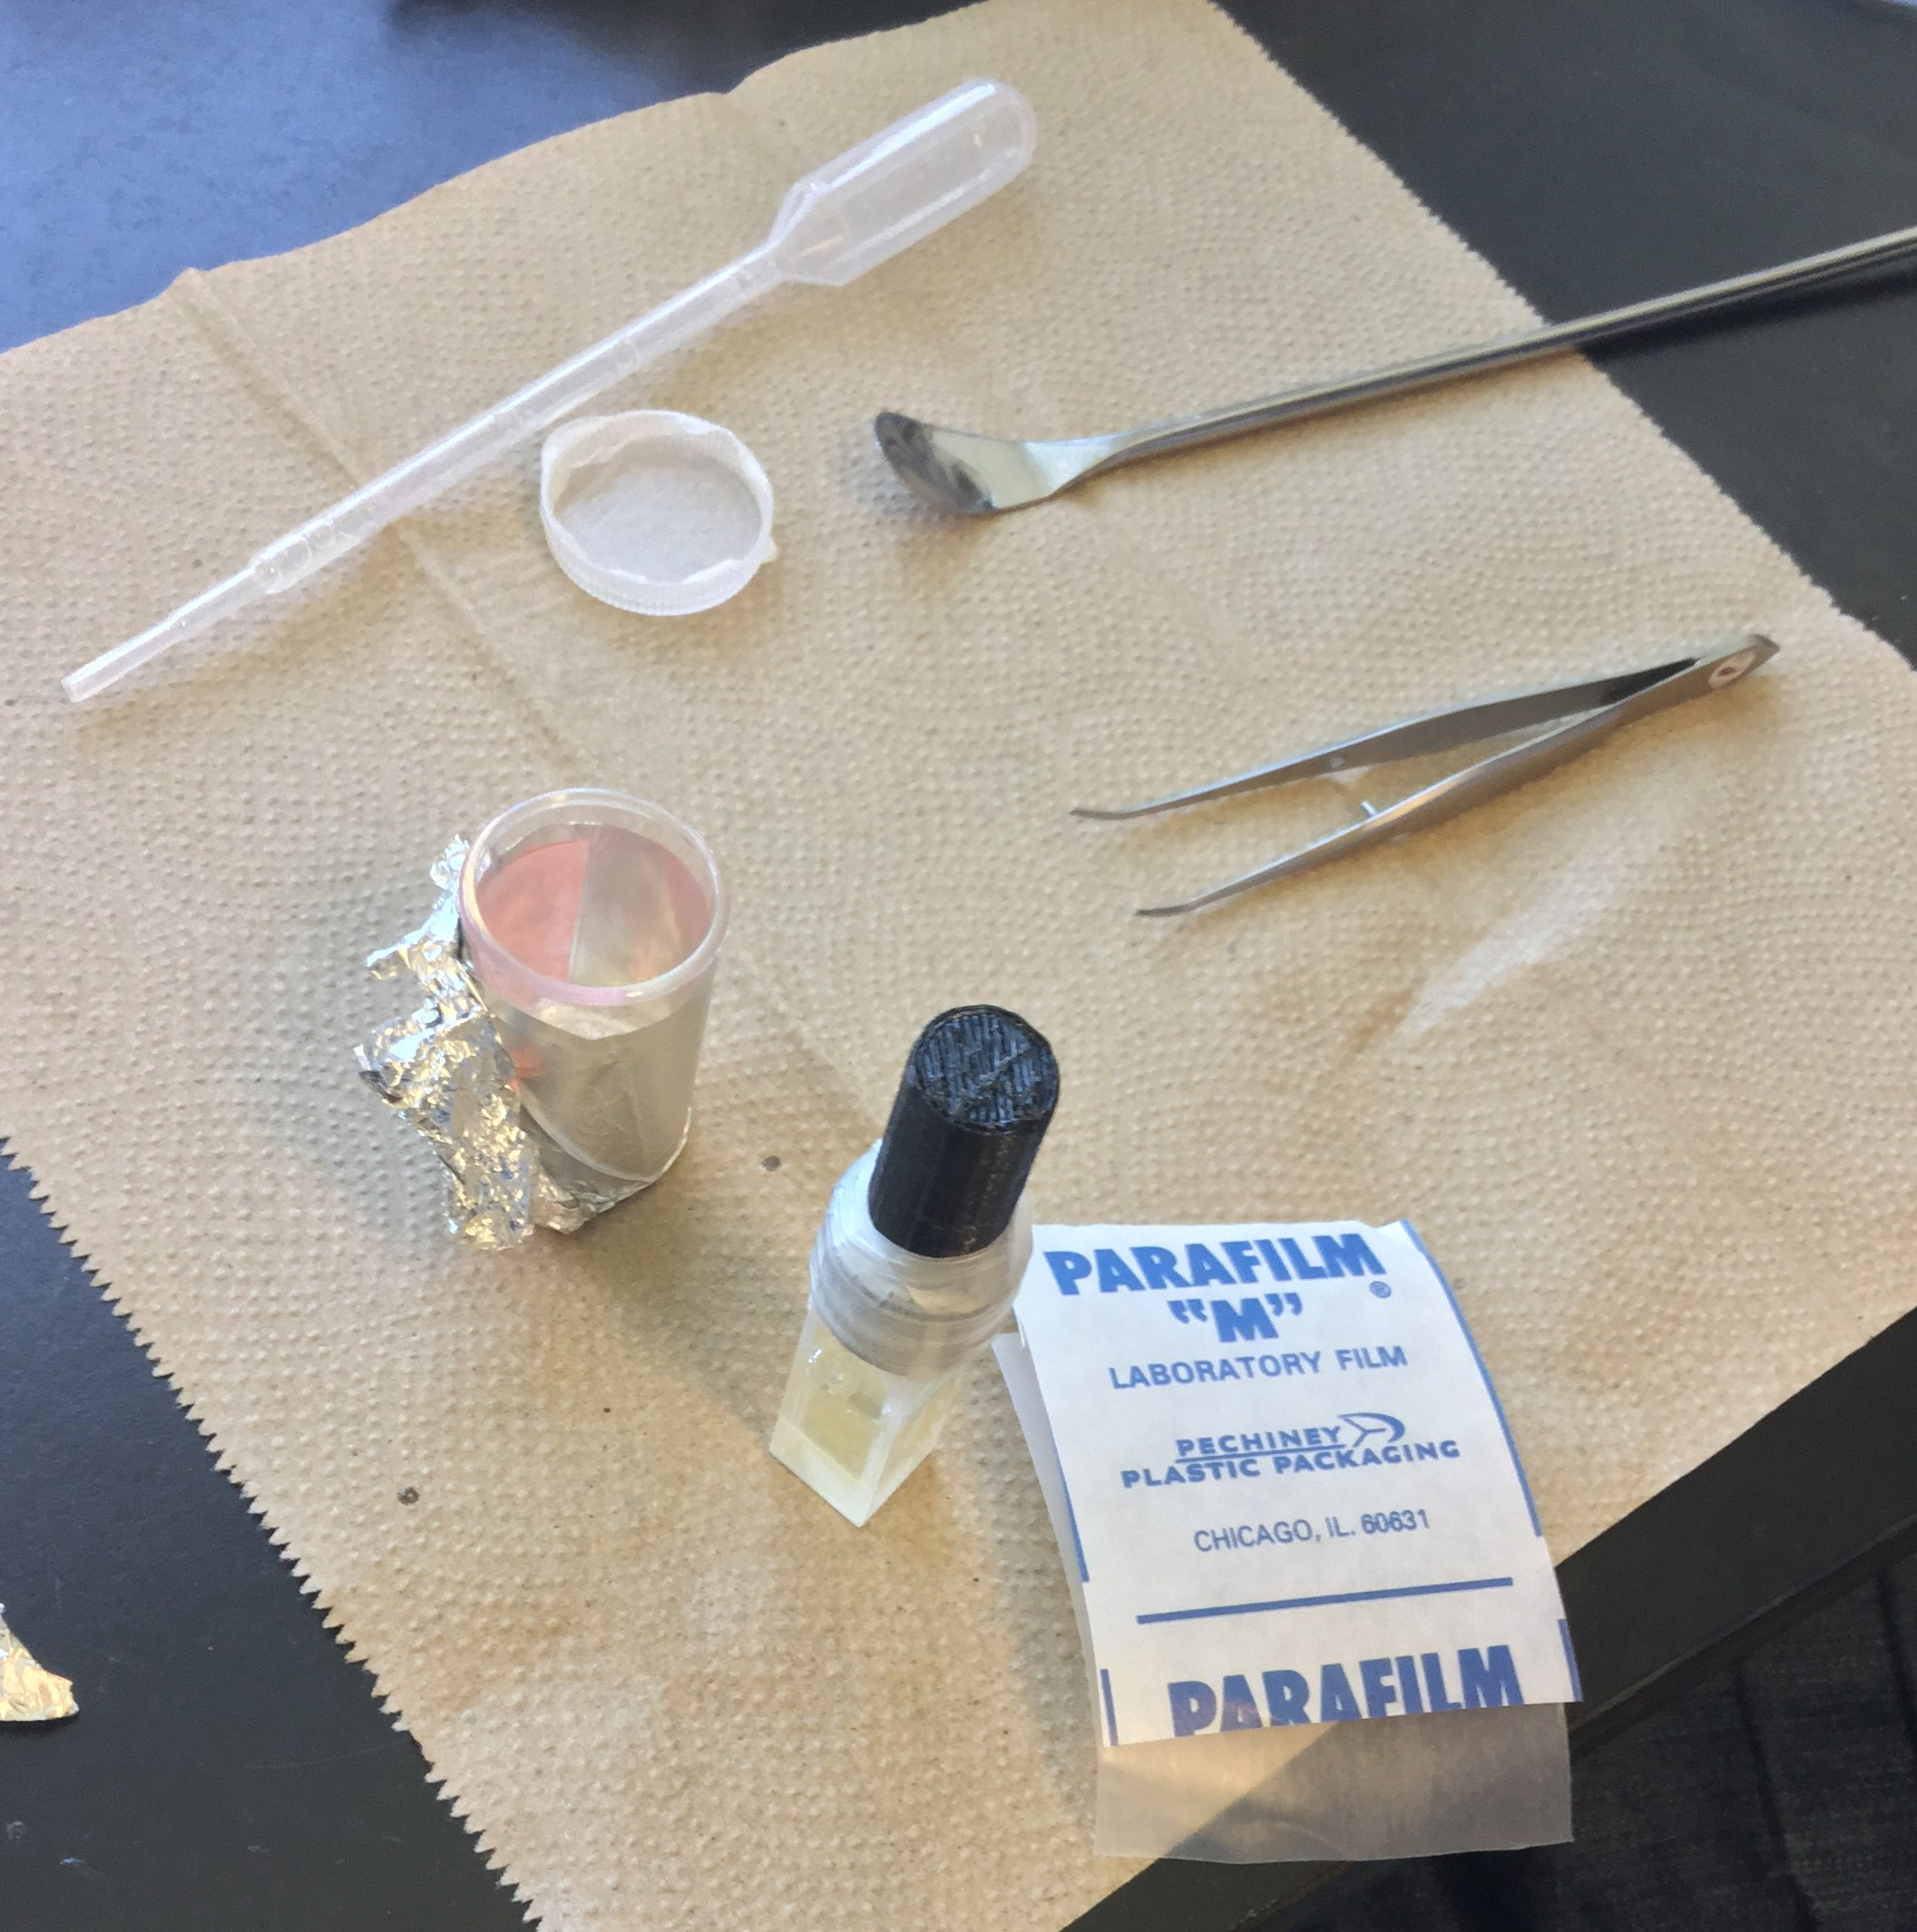
\includegraphics[width=6cm]{parafilm.jpg}
        \caption{Préparation de la cuvette}
        \label{fig:parafilm}
        \end{figure}
\end{enumerate}
\subsection{Installer l'échantillon sur le microscope}
\begin{enumerate}
    \item Retirer la cuvette de liquide fluorescent. L'essuyer avec soin.
    \item Retirer l'eau de la chambre à l'aide d'une pipette.
    \item Remplir la chambre du liquide approprié\footnote{Le liquide de la chambre doit avoir le même indice de réfraction que l'échantillon (et que la solution dans laquelle beigne l'échantillon). Par exemple, pour un cerveau soumis à la méthode \textit{Clarity}, on peut utiliser du glycérol (n=1.47). Pour la méthode \textit{Idisco}, on peut utiliser de l'Éthyl cinnamate (n=1.52). [Attention:~Puisque l'Éthyl cinnamate a une structure moléculaire très semblable à celle du plastique, il a tendance à fuir de la chambre et à s'infiltrer dans l'objectif, ce qui finit par l'endommager grandement à long terme.]}.
    \item \label{observations} Répéter les étapes \ref{ref1} à \ref{ref2} de la section~\ref{ssec:aligner_la_cam} avec la cuvette contenant l'échantillon à imager.
    \\ Note: Avant d'installer l'échantillon sur le microscope, bien étudier sa forme et l'orientation à laquelle on le place par rapport au montage. Au besoin, se faire un dessin. Ces observations seront très utiles lorsqu'il sera temps de \textit{Saisir les paramètres de scan 3D}.
    
    \item Changer le filtre (voir figure~\ref{fig:filtres}) si nécessaire.
    \item Mettre la couverture noire comme sur la figure~\ref{fig:couverture}. Attention: La couverture ne doit pas se retrouver sur le parcours du laser!
        \begin{figure}[H]
        \centering
        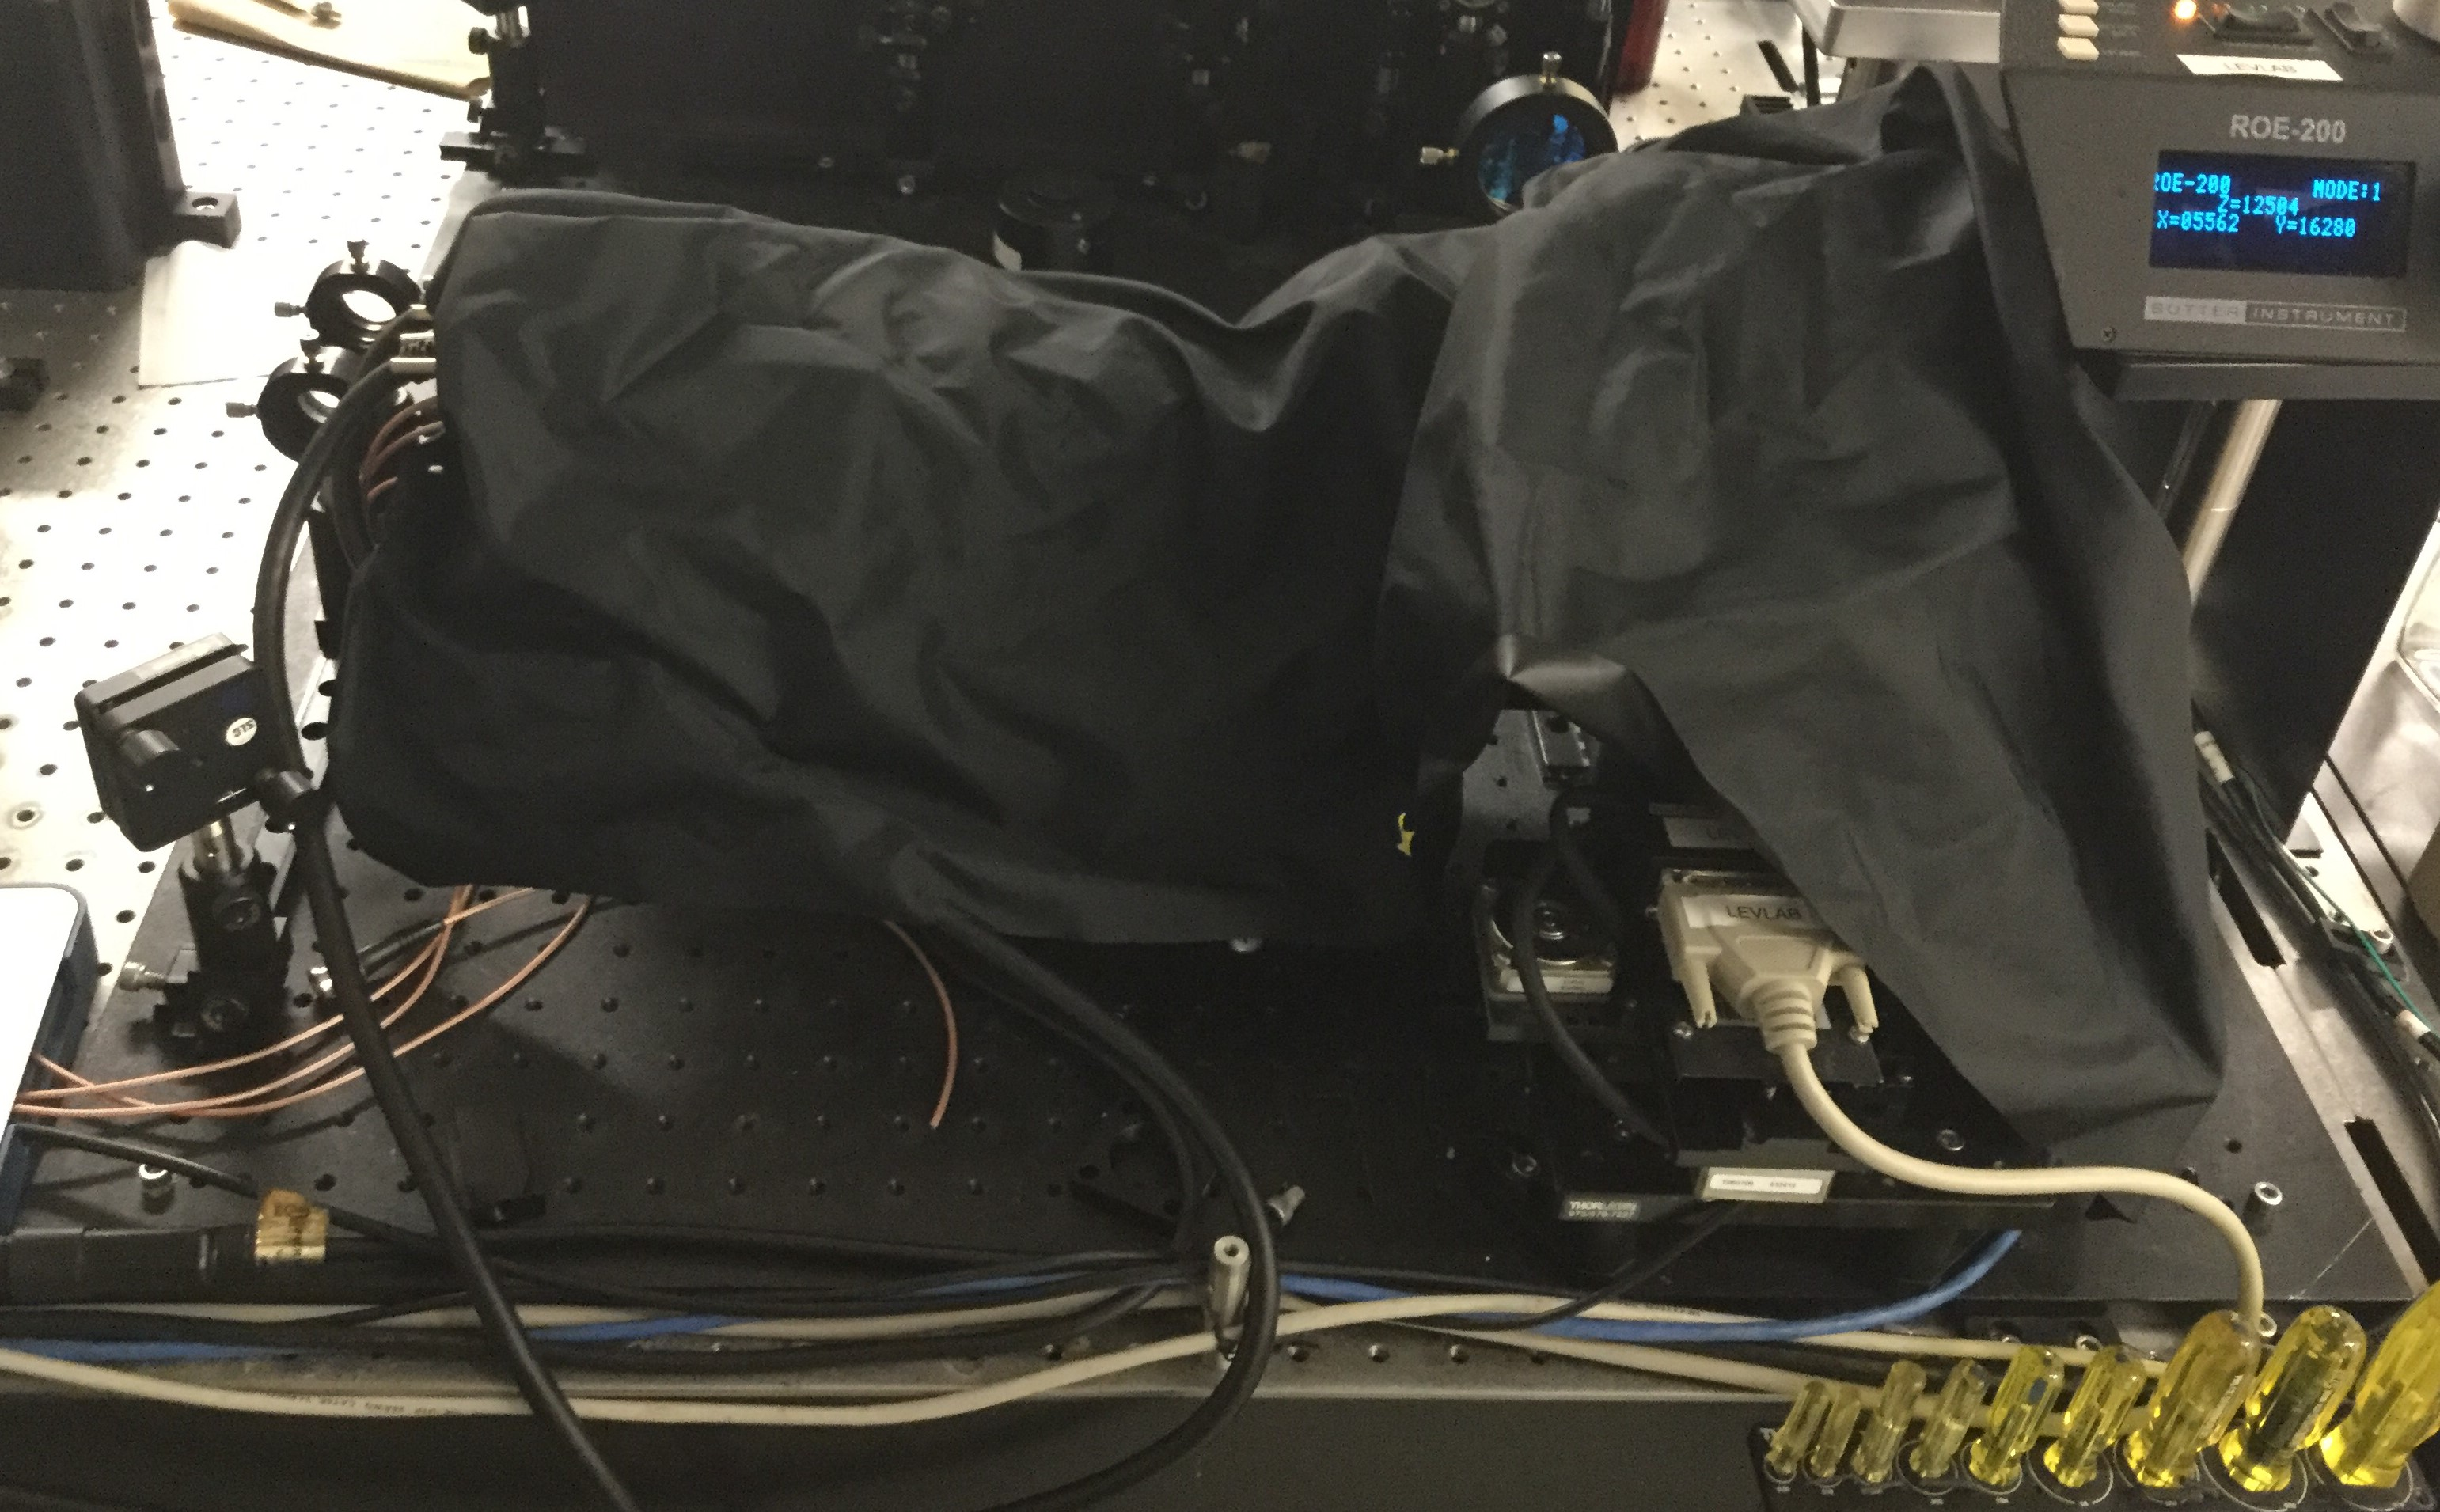
\includegraphics[width=8cm]{couverture.jpg}
        \caption{Couverture sur le montage}
        \label{fig:couverture}
        \end{figure}
    
    \item Cliquer sur \textit{Scan. and Trig.} (6e bouton).
    \item Cliquer sur le menu déroulant indiqué à la figure~\ref{fig:tiret}. Sélectionner l'option '-'. Cliquer sur X pour fermer la fenêtre.
    \item Au besoin, ajuster le contraste.
   \item Ajuster la position en profondeur de la caméra à l'aide la \textit{vis C} (voir figure~\ref{fig:vis}).
    \\ But: Avoir la ligne de fluorescence au focus, i.e. avoir la ligne la plus nette/fine possible.
    \item Utiliser les outils d'alignement si nécessaire.
    \item Remettre à l'option '$\uparrow\downarrow$'.
\end{enumerate}
\subsection{Saisir les paramètres de scan 3D}
\begin{enumerate}
    
    \item Sur l'interface d'accueil (voir figure~\ref{fig:accueil}), cliquer sur \textit{CFG Experiment} (7e bouton).
    \item \label{extremums1} Tourner la \textit{roulette de devant} (voir figure~\ref{fig:roulettes}) dans le sens antihoraire jusqu'à atteindre le rebord de l'échantillon, i.e. perdre du signal de fluorescence à l'écran. Il s'agit d'un extremum local mais peut-être pas de l'extremum global.
    \item En se souvenant des observations notées à l'étape~\ref{observations}, tourner un peu la \textit{roulette du dessus}, puis réajuster la \textit{roulette de devant} pour retrouver l'extremum local. Le but est d'avoir la valeur la plus petite possible pour la \textit{roulette de devant}. Les valeurs des roulettes sont affichées comme sur la figure~\ref{fig:roulettes}. Itérer jusqu'à retrouver l'extremum global.
    \item Refaire le même processus, mais en ajustant la \textit{roulette de devant} par rapport à la \textit{roulette de droite}.
    \item \label{extremums2} Une fois la valeur minimale trouvée, cliquer sur \textit{Width LO} (voir figure~\ref{fig:cf}).
        \begin{figure}[H]
        \centering
        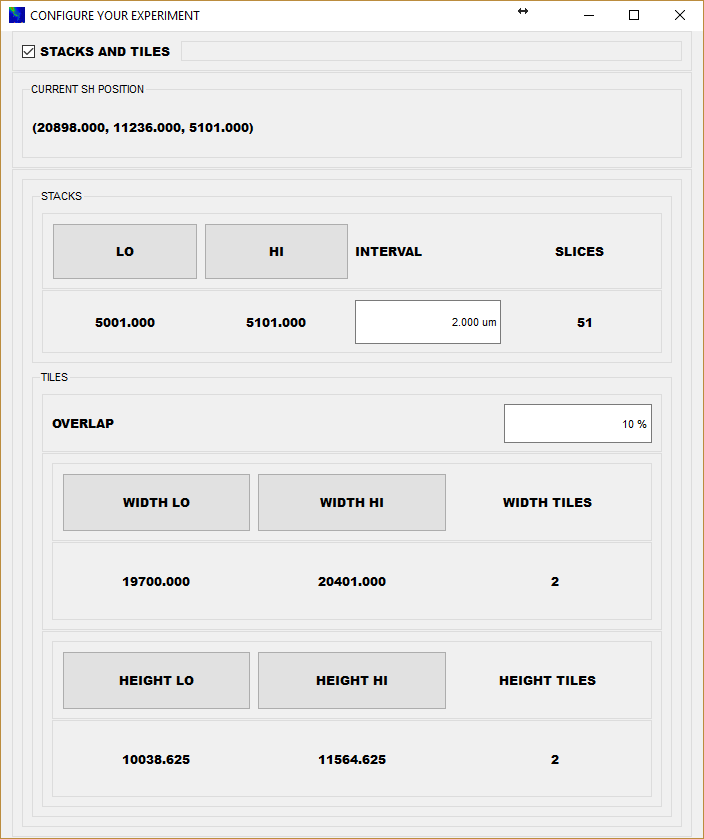
\includegraphics[width=10cm]{cf.png}
        \caption{Fenêtre pop-up de \textit{CFG Experiment}}
        \label{fig:cf}
        \end{figure}
    \item Refaire les étapes~\ref{extremums1} à \ref{extremums2} en suivant l'ordre suivant:
        \begin{itemize}
        \item[$\bullet$] Pour \textit{Width HI}: \textit{roulette de devant} p/r à \textit{roulette de dessus}, puis p/r à \textit{roulette de droite}
        \item[$\bullet$] Pour \textit{Height LO}: \textit{roulette de dessus} p/r à \textit{roulette de devant}, puis p/r à \textit{roulette de droite}
        \item[$\bullet$] Pour \textit{Height HI}: \textit{roulette de dessus} p/r à \textit{roulette de devant}, puis p/r à \textit{roulette de droite}
        \end{itemize}
    *** Les valeurs choisies pour chaque extremum sont gardées en mémoire et affichées sous leur bouton respectif.
    \item Mettre la \textit{roulette de devant} sur la valeur calculée de la façon suivante:
    $$ roulette~de~devant = \frac{valeur~de~Width~HI - valeur~de~Width~LO}{2} + valeur~de~Width~LO $$
    \item Mettre la \textit{roulette du dessus} sur la valeur calculée de la façon suivante:
    $$ roulette~du~dessus = \frac{valeur~de~Height~HI - valeur~de~Height~LO}{2} + valeur~de~Heigth~LO $$
    \item Tourner la \textit{roulette de droite} (voir figure~\ref{fig:roulettes}) dans le sens antihoraire jusqu'à atteindre le rebord de l'échantillon, i.e. perdre du signal de fluorescence à l'écran. Cliquer sur \textit{LO}.
    \item Tourner la \textit{roulette de droite} dans le sens horaire jusqu'à atteindre le rebord de l'échantillon, i.e. perdre du signal de fluorescence à l'écran. Cliquer sur \textit{HI}.
    \item Vérifier que l'intervalle entre chaque stack est de 2.000 um (par défaut) ou plus.
    \item Vérifier que le pourcentage d'overlap est entre 10\% (par défaut) et 20\%.
    \item Cliquer sur X pour fermer la fenêtre.
\end{enumerate}
\subsection{Lancer l'acquisition de données}
\label{start}
\begin{enumerate}
    \item Sur l'interface d'accueil (voir figure~\ref{fig:accueil}), cliquer sur \textit{Camera}.
    \item Sélectionner le \textit{Binning} voulu: 1~=~image plus précise, acquisition plus lente. 4~=~image moins précise, acquisition plus rapide.
    \item Définir l'\textit{Exposure} voulu: valeur plus grande~=~plus de signal détecté par la caméra, acquisition plus lente. Toujours choisir une valeur de 80~ms ou plus.
    \item Cliquer sur X pour fermer la fenêtre.
    \item Cliquer sur \textit{Stop} (bouton rouge).
    \item Cliquer sur \textit{Start Experim.}.
\end{enumerate}
L'acquisition prend un certain temps, dépendamment de la grosseur de l'échantillon et des paramètres de scan choisis. Un cerveau complet de souris peut prendre jusqu'à 10~heures. Pour évaluer le temps d'acquisition: $$dur\acute{e}e~de~l'acquisition = nb~de~slices \cdot nb~de~width~tiles \cdot nb~de~height~tiles \cdot temps~d'exposition$$ Les trois premiers paramètres se retrouvent dans \textit{CFG Experiment}. Le dernier paramètre se retrouve dans \textit{Camera} à \textit{Exposure}.
\\ \\
De plus, il se peut que l'erreur montrée à la figure~\ref{fig:sauce} se produise. Normalement, le problème se règle par lui-même. Cependant, si la fenêtre demeure affichée plus de 15 secondes, il faut éteindre le contrôleur du \textit{sutter ROE-200} (voir figure~\ref{fig:sutter}), attendre quelques secondes et le rallumer.
%
\begin{figure}[H]
%
\begin{minipage}{0.45\textwidth}
\centering
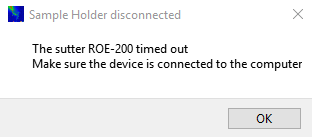
\includegraphics[width=7cm]{sauce.PNG}
\caption{Message d'erreur du \textit{sutter}}
\label{fig:sauce}
\end{minipage}
%
\hfill
%
\begin{minipage}{0.45\linewidth}
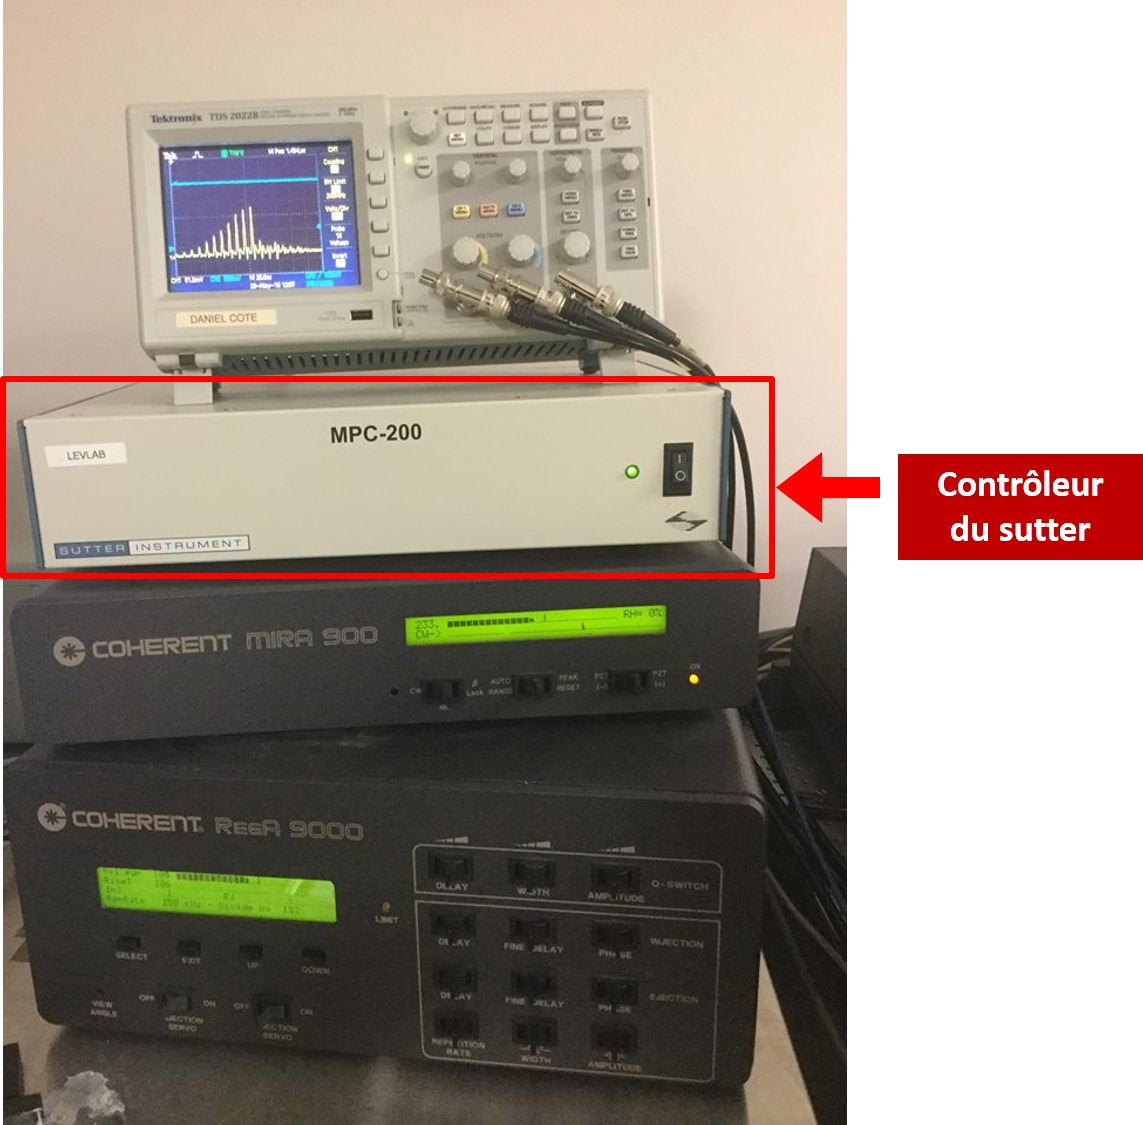
\includegraphics[width=7cm]{sutter.png}
\caption{Contrôleur du \textit{sutter}}
\label{fig:sutter}
\end{minipage}
%
\end{figure}

\section{\textcolor{magenta}{Procédure de fermeture du lab}}


\begin{enumerate}
    \item Replacer le \textit{beam dump} devant la sortie du laser (voir figure~\ref{fig:beam-dump}).
    \item Sur le \textit{contrôleur du Verdi}, peser sur le bouton \textit{Shutter Open} (voir figure~\ref{fig:controleur-verdi}). On peut maintenant enlever les lunettes de sécurité.
    \item Sur l'interface d'accueil du logiciel \textit{Umoco}, cliquer sur X. Confirmer l'arrêt du logiciel \textit{Umoco}.
    \item Éteindre la caméra: mettre l'interrupteur \textit{Power} de \textit{On} à \textit{Off} (voir figure~\ref{fig:cam_power}).
\begin{center} $\ast\ast\ast$ Si vous avez d'autres échantillons à imager dans les prochains jours, passez tout de suite à l'étape~\ref{skip}. Puisque l'ouverture complète du laser peut être longue, on peut le laisser à \textit{On} quelques jours consécutifs. Il faut alors laisser la lumière rouge d'avertissement allumée.  $\ast\ast\ast$ \end{center}
    \item Tourner la clé de \textit{On} à \textit{Standby} sur le \textit{contrôleur du Verdi} (voir figure~\ref{fig:controleur-verdi}).
    \item Sur le \textit{contrôleur du Verdi}, aller dans \textit{LBO Settings} et mettre le \textit{'LBO'} sur l'état \textit{'Cooling'}. Peser deux fois sur \textit{Menu Exit}.
    \item Tourner la roulette pour atteindre une puissance de 0~W.
    \item \textcolor{magenta}{HELLO}
    \item Sur chaque refroidisseur (voir figure~\ref{fig:cooler}), peser sur le bouton \textit{Run/Standby}. Le message \textit{Standby Mode} devrait s'afficher.
    \item Derrière le \textit{contrôleur du Verdi}, mettre la bascule sur \textit{Off}.
    \item Sur le \textit{contrôleur du Mira} (voir figure~\ref{fig:controleurs}), mettre la bascule de gauche sur \textit{CW}.
    \item Éteindre la lumière rouge d'avertissement grâce à l'interrupteur \textcolor{magenta}{FIGURE}.
    \item \label{skip} Retirer la cuvette contenant l'échantillon.
    \item Retirer le liquide de la chambre à l'aide d'une pipette. Ce liquide est généralement réutilisable et peut être conservé dans un contenant à part.
    \item Rincer l'intérieur de la chambre à l'aide d'un flacon laveur d'eau (voir figure~\ref{fig:eau}).
    \item A l'aide d'une autre pipette, transvider les restants de liquides dans le bécher à déchets.
    \item Répéter les deux dernières étapes si nécessaire.
    \item Prendre un papier optique (voir figure~\ref{fig:papier}). Le plier jusqu'à grandeur voulue. Prendre soin de ne jamais toucher la partie du papier optique qui entrera en contact avec l'objectif. 
        \begin{figure}[H]
        \centering
        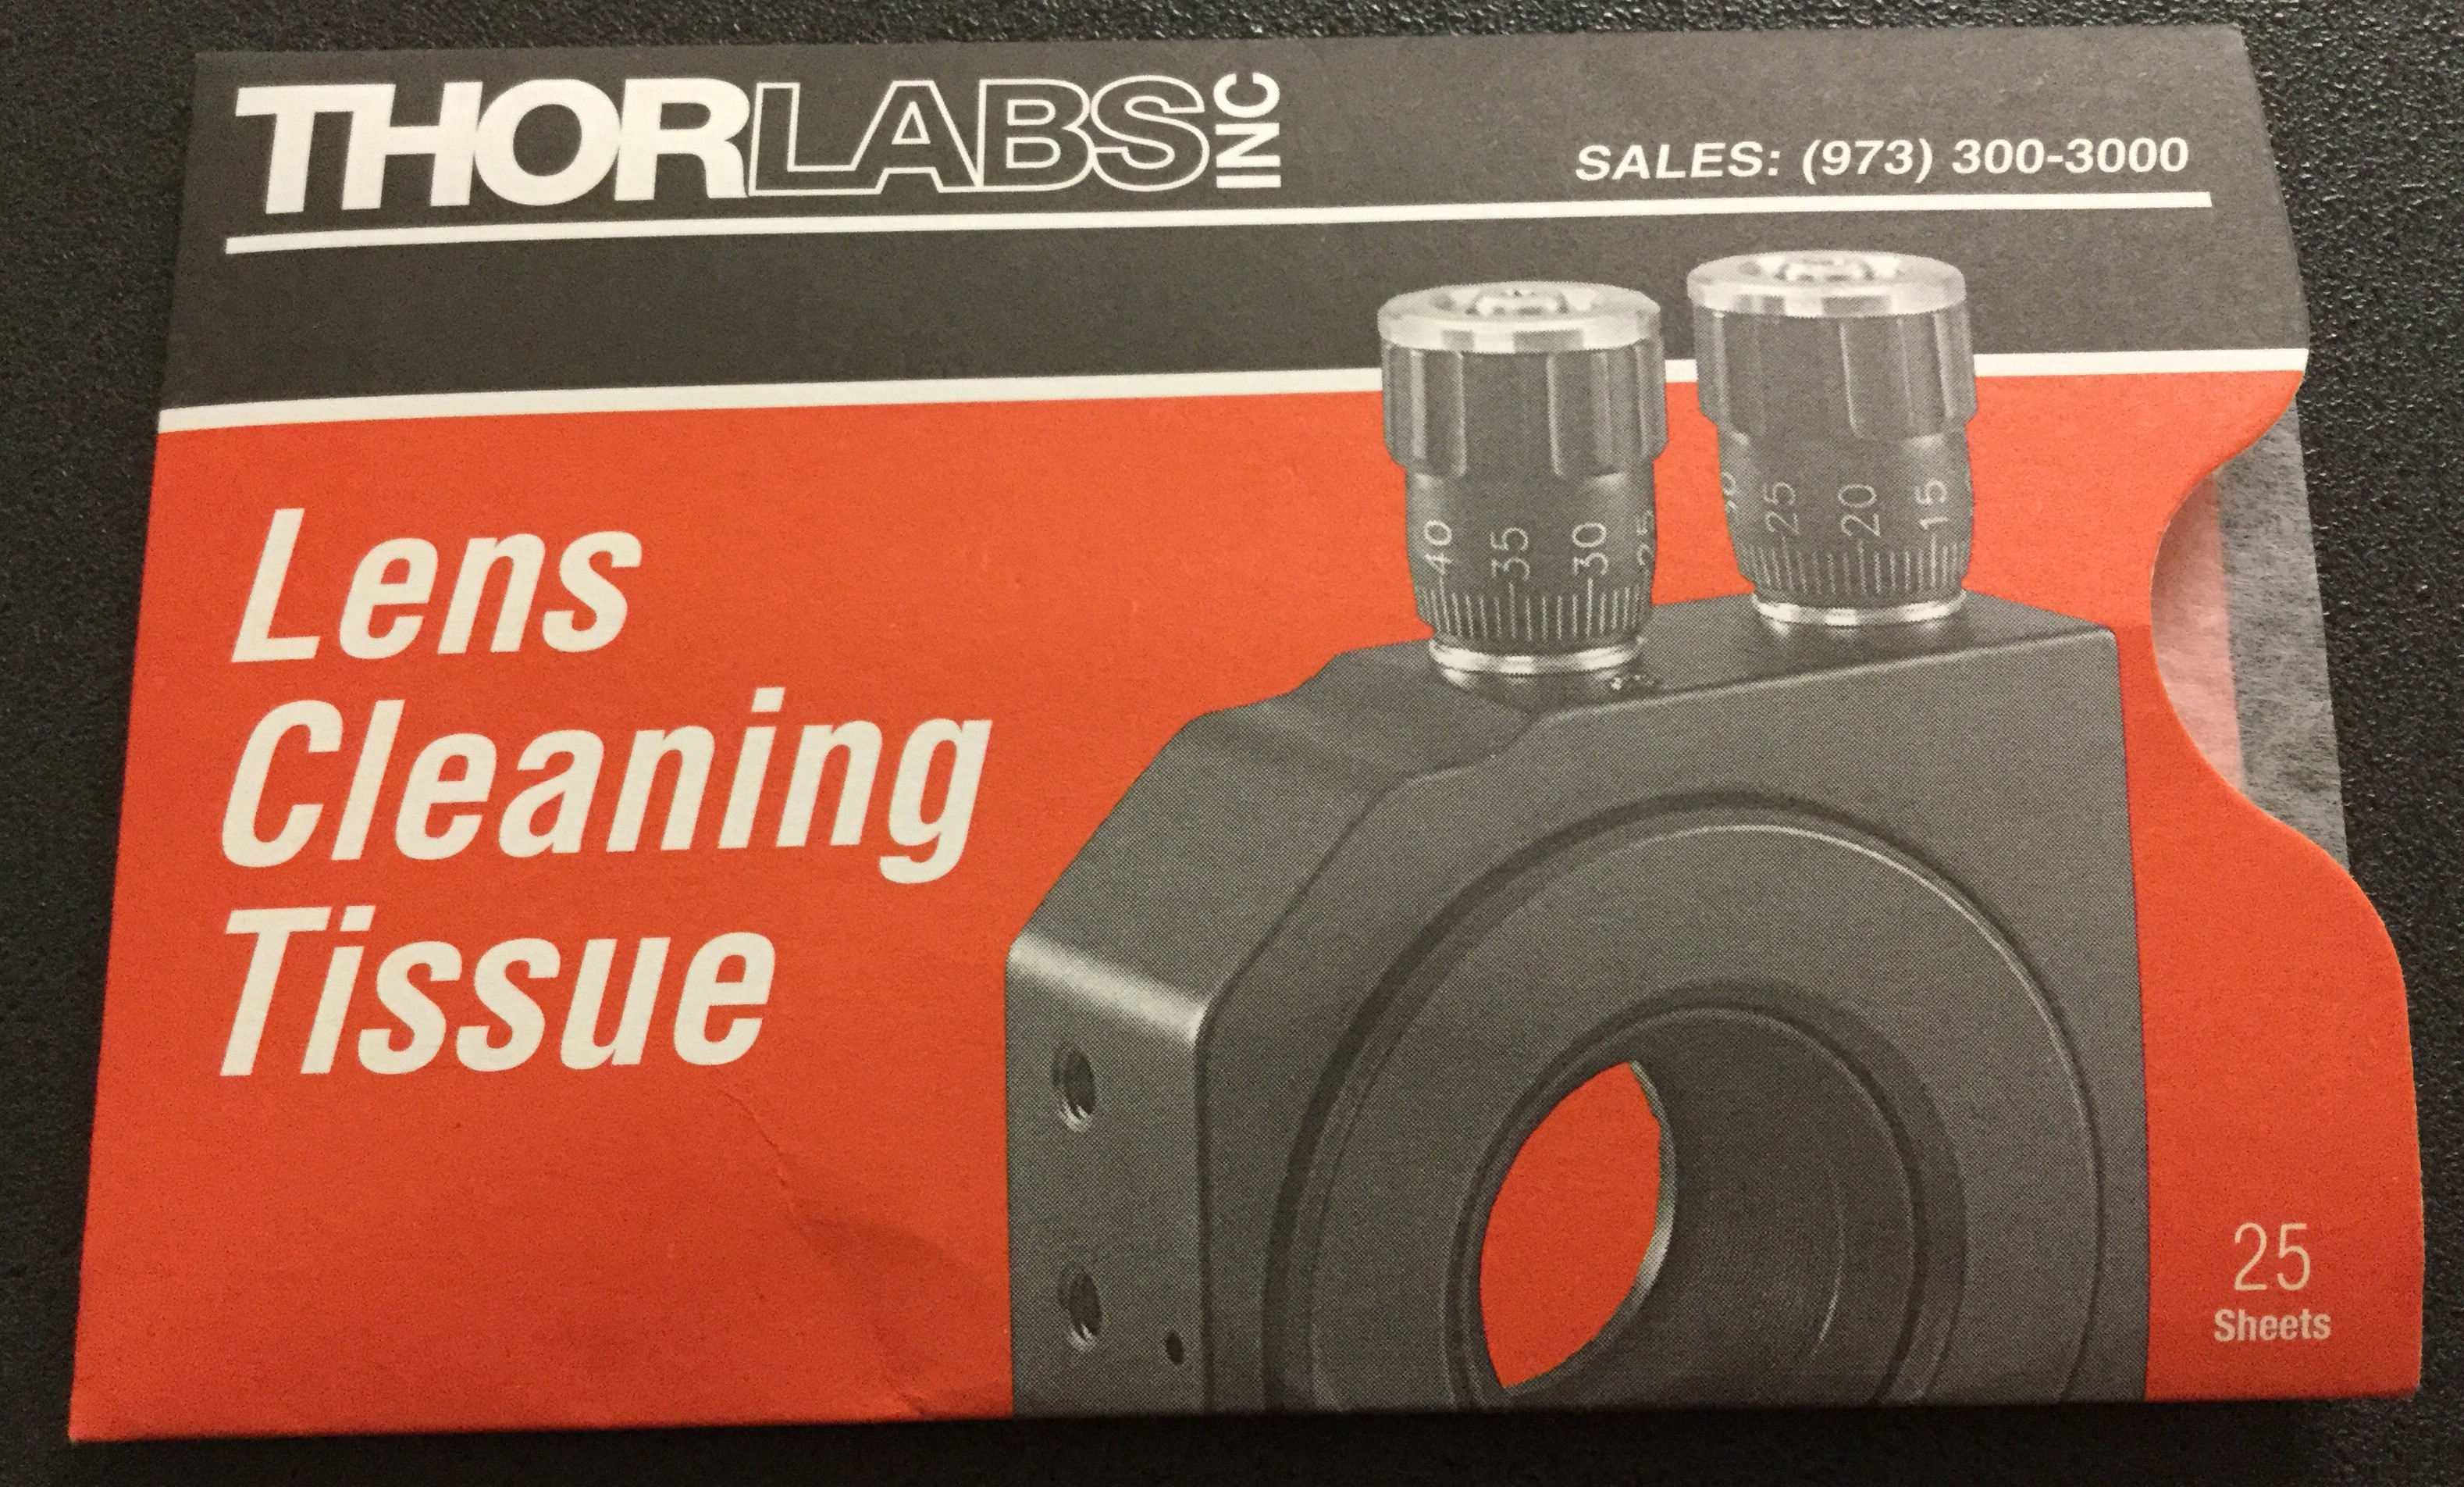
\includegraphics[width=5cm]{papier.jpg}
        \caption{Papier optique}
        \label{fig:papier}
        \end{figure}
    \item Passer doucement le papier sur l'objectif, et ce, une seule fois (pas d'aller-retour). Ne pas mettre de pression. Jeter le papier.
    \item Répéter les deux dernière étapes si nécessaire. Ne jamais utiliser deux fois le même papier optique.
    \item Au besoin, mettre des gants et utiliser un peu d'éthanol avec le papier optique.
    \item Remettre l'échantillon dans son contenant d'origine.
    \item Mettre des gants. Nettoyer la cuvette avec de l'éthanol. \item Si la cuvette est en verre: Laisser sécher à l'air libre. Ne pas essuyer.
\end{enumerate}

\section{Traitement et visualisation des données}
\subsection{Stitching}
Une fois l'acquisition terminée, le fichier de données se trouve dans le répertoire déterminé à la section \ref{start}. Afin de 'stitcher' (assembler les tuiles) les données, il faut ouvrir l'application MATLAB se trouvant dans la barre de tâches.


\begin{figure}[H]
    \centering
    
\includegraphics[scale = 0.7]{taskbar.png}
    \caption{Ouvrir MATLAB}
    \label{fig:task_bar}
\end{figure}

Une fois MATLAB ouvert, assurez-vous que vous êtes bien dans le répertoire 'LightsheetUtilities', comme à la figure~\ref{fig:repertpoire}.

\begin{figure}[H]
    \centering
    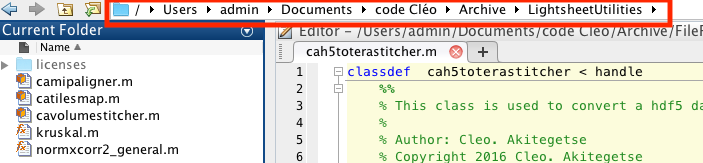
\includegraphics[scale = 0.7]{repertoire.png}
    \caption{Répertoire LightsheetsUtilities}
    \label{fig:repertpoire}
\end{figure}

\begin{figure}[H]
    \centering
    \subfloat{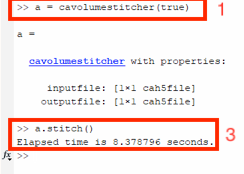
\includegraphics[width=6cm]{1-3.png} }%
    \qquad
    \subfloat{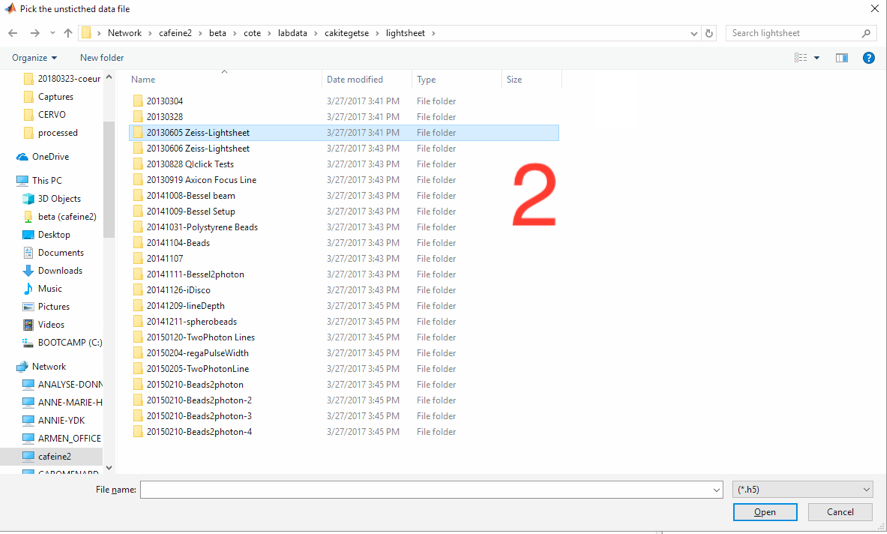
\includegraphics[width=9cm]{2.png} }%
    \caption{Les 3 étapes pour 'stitcher' les données}%
    \label{fig:cmd}%
\end{figure}

Exécutez la commande suivante (1) dans la fenêtre de commande de MATLAB.
$$>>a = cavolumestitcher(true) $$

Comme illustré à la figure \ref{fig:cmd}, une fenêtre apparaîtra afin que l'utilisateur puisse sélectionner  les données qu'il aimerait 'stitcher'. Une fois le fichier sélectionné, les informations sur celui s'afficheront dans la fenêtre de commande. Afin de terminer le traitement des données, l'utilisateur doit entrez la commande suivante (3):
$$>>a.stitch()$$

Cette opération peut être longue dépendamment de la grosseur du fichier. Une barre de progression sera affichée à l'écran. Le fichier créer par cette dernière étape sera enregistré dans le même répertoire que le fichier d'origine contenant les données non traitées.

\subsection{Visualisation 3D}
Afin de visualiser les données, ouvrez l'application 'Vaa3D' se trouvant dans la barre de tâches.

\begin{center}\textcolor{red}{***Attention! Assurez vous qu'aucun fichier temporaire du genre 'vmap.bin' se trouve dans le répertoire dans lequel se trouve le fichier que vous désirez ouvrir. En présence d'un tel fichier, supprimez-le. ***}\end{center}


\begin{figure}[H]
    \centering
    
\includegraphics[scale = 0.7]{taskbar2.png}
    \caption{Ouvrir Vaa3D}
    \label{fig:vaad}
\end{figure}

Une fois l'application en ouverte, lancez le plugin TeraFly en suivant les étapes de la figure~\ref{fig:big}.

\begin{figure}[H]
    \centering
    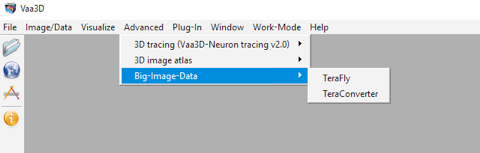
\includegraphics[scale = 0.7]{big.png}
    \caption{ Ouverture du plugin TeraFly}
    \label{fig:big}
\end{figure}

À partir de TeraFly, vous pouvez ouvrir le fichier que vous venez de traiter en suivant les étapes de la figure~\ref{fig:tera}.

\begin{figure}[H]
    \centering
    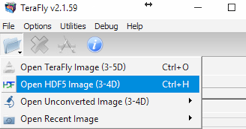
\includegraphics[scale = 1]{tera.png}
    \caption{Ouverture de fichier via TeraFly}
    \label{fig:tera}
\end{figure}

Les données seront visibles sous forme d'un volume. Il est possible de naviguer dans le volume et d'agrandir certaine section.

\appendix
\newpage
\section{Protocole - Remplacer l'eau des chillers}
\label{a:chillers}

\textbf{N.B. Prévoir un seau pour vider les conduits et le chiller pour ne pas inonder le laboratoire. Traitement à effectuer tous les 3 mois.}

\subsection*{Remplacer l'eau des conduits}
Remplacer l'eau du chiller ne suffit pas à retirer toute l'eau du système. De l'eau s'est également accumulée dans les conduits des cavités laser et il faut les vider.
\begin{enumerate}
\item Éteindre le laser si ce n'est pas déjà fait
\item Éteindre le chiller
\item Retirer les tuyaux et les déposer dans un contenant pour recueillir l'eau des conduits
\item Vider le chiller de son eau
\item Mettre 400 ml d'eau doublement distillée (très important de mettre l'eau désionisée et déminéralisée)
\item Reconnecter le tout et rallumer le chiller
\item Laisser tourner l'eau pendant une dizaine de minutes
\item Répéter 1-2 fois
\end{enumerate}

\subsection*{Produit anticorrosif}
Le produit anticorrosif provient de la compagnie "OptiTemp". Le produit est OptiShield Plus. C'est un produit spécifiquement fait pour protéger les circuits d'eau fermés de la corrosion. Il protège des contaminants que contiennent l'aluminium, le bronze, le cuivre et tout type de métaux si ceux-ci sont présents dans le circuit. Une photo mise à la fin du document donne une description du produit.
\begin{enumerate}
\item Prendre environ 40 ml du produit anticorrosif
\item Ajouter 400 ml d'eau désionisée et déminéralisée (doublement distillé)
\item Remplir le chiller avec la solution
\item Allumer le chiller et laisser remplir les tuyaux de la solution
\item Ajouter le reste de la solution s'il en reste (le niveau d'eau a diminué pour remplir les conduits de la cavité laser)
\end{enumerate}

\begin{figure}[t!]
\centering
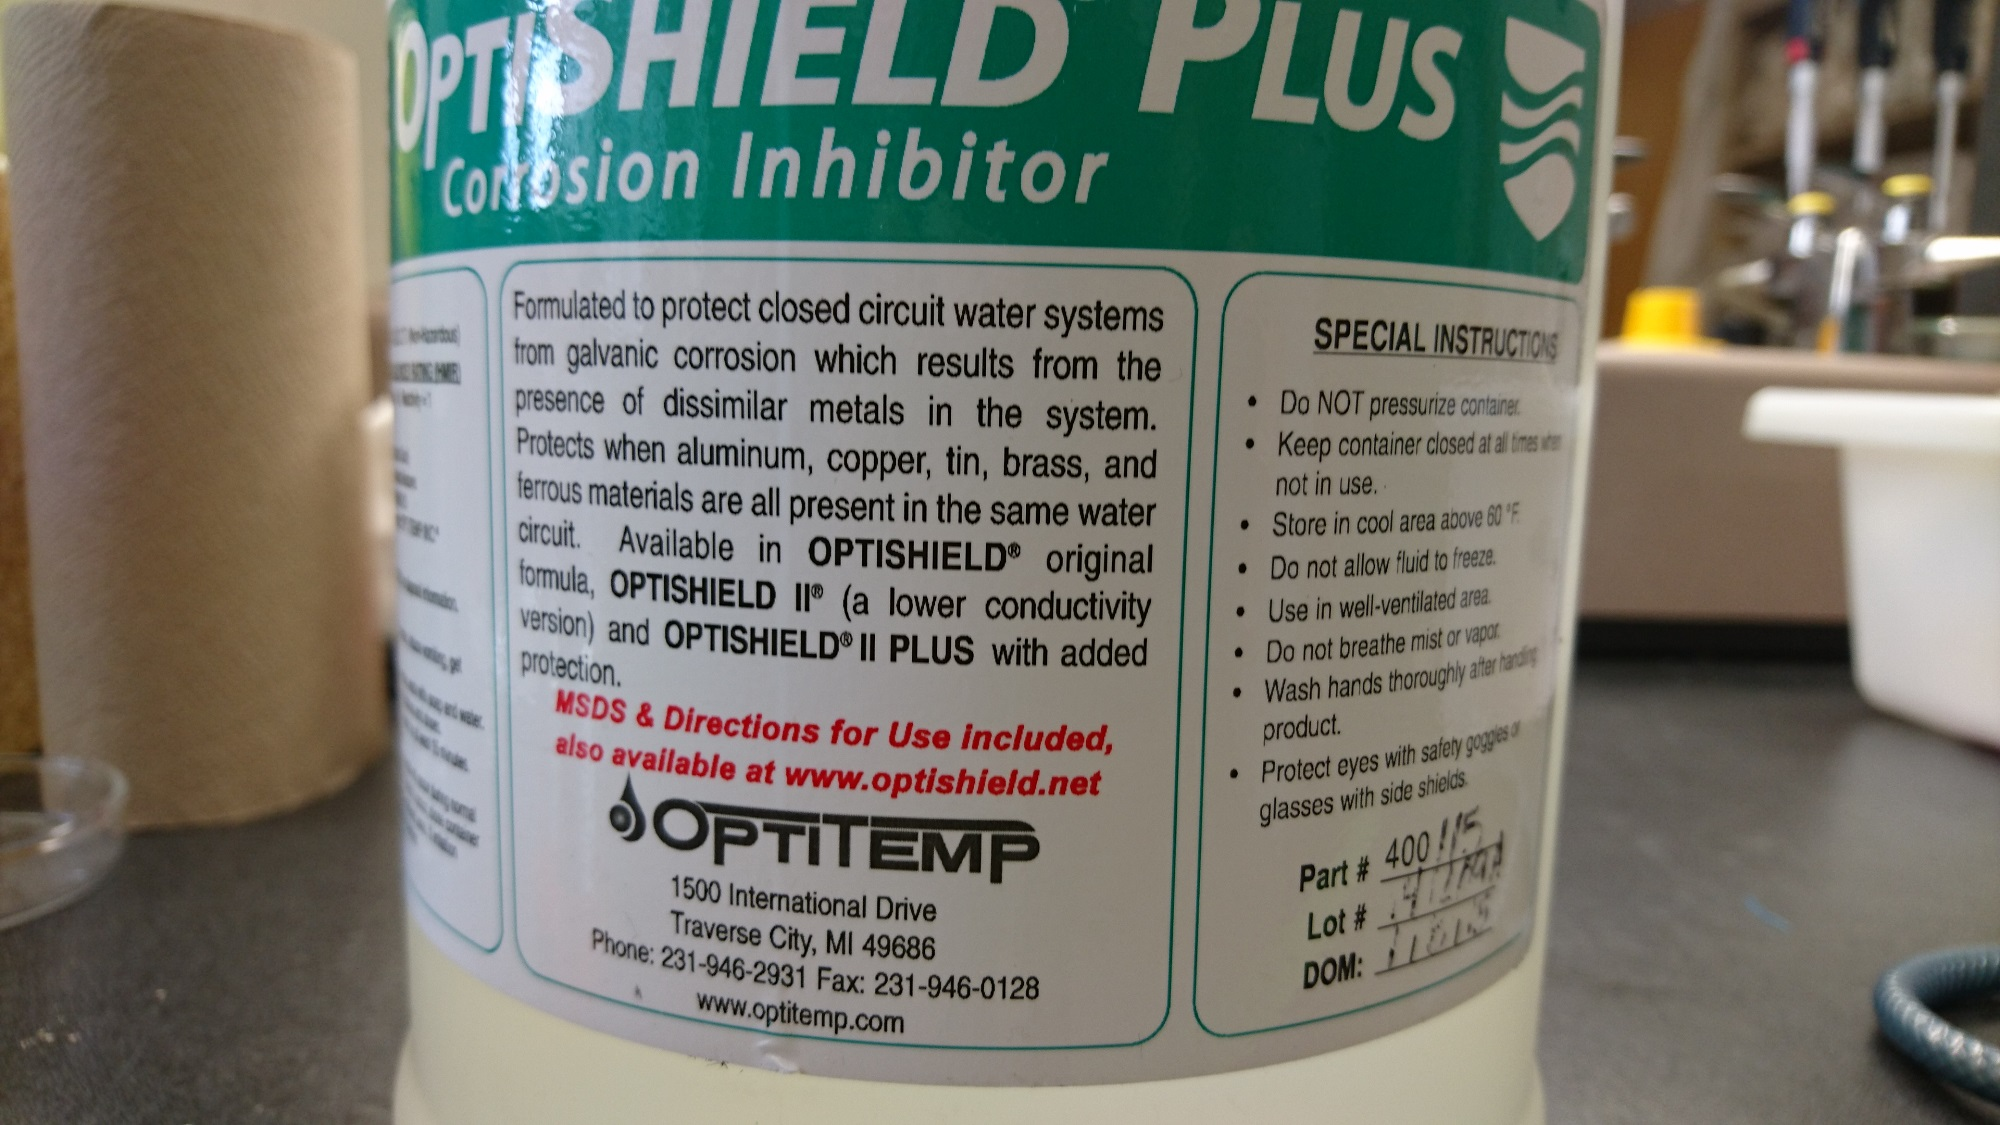
\includegraphics[scale=0.2]{anticorrosif_chiller.jpg}
\end{figure}

\end{document}


